% concatenated from main.tex
\documentclass[11pt,oneside]{amsart}
\usepackage{amsmath,amsfonts,amsthm,amssymb}
\usepackage{MnSymbol}
\usepackage{tikz}
\usetikzlibrary{arrows,decorations.pathmorphing,backgrounds,positioning,fit,calc}
\usepackage{setspace}
\onehalfspacing
\usepackage{fullpage}
\usepackage{hyperref}
\usepackage[subrefformat=parens, labelfont=up]{subcaption}

\newtheorem{thm}{Theorem}
\newtheorem*{mthm}{Main Theorem}

%for restating theorem with custom numbering
\newtheorem{innercustomthm}{Theorem}
\newenvironment{rethm}[1]
  {\renewcommand\theinnercustomthm{#1}\innercustomthm}
  {\endinnercustomthm}
%\begin{rethm}{\ref{theorem}} or \begin{rethm}{custom number}
%\end{prethm}

\newtheorem{lemma}[thm]{Lemma}
\newtheorem{conj}[thm]{Conjecture}
\newtheorem{coro}[thm]{Corollary}
\newtheorem{prop}[thm]{Proposition}
\newtheorem{claim}[thm]{Claim}
\theoremstyle{definition}
%\newtheorem{defn}[thm]{Definition}
\theoremstyle{remark}
%\newtheorem{rem}[thm]{Remark}
%\newtheorem{ex}[thm]{Example}

\newenvironment{ex}{\refstepcounter{thm}\begin{proof}[Example \emph{\thethm}]\renewcommand*{\qedsymbol}{\(\blacksquare\)}}{\end{proof}}
\newenvironment{rem}{\refstepcounter{thm}\begin{proof}[Remark \emph{\thethm}]\renewcommand*{\qedsymbol}{\(\blacksquare\)}}{\end{proof}}
\newenvironment{defn}{\refstepcounter{thm}\begin{proof}[Definition \emph{\thethm}]\renewcommand*{\qedsymbol}{\(\blacksquare\)}}{\end{proof}}
\newenvironment{quest}{\refstepcounter{thm}\begin{proof}[Question \emph{\thethm}]\renewcommand*{\qedsymbol}{\(\blacksquare\)}}{\end{proof}}
\newenvironment{warn}{\refstepcounter{thm}\begin{proof}[Warning \emph{\thethm}]\renewcommand*{\qedsymbol}{\(\blacksquare\)}}{\end{proof}}
\numberwithin{equation}{section}

\setcounter{tocdepth}{3} 

\pagestyle{empty}

%\setlength{\textwidth}{390pt}
%\setlength{\oddsidemargin}{45pt}
%\setlength{\evensidemargin}{45pt}

\def\CC{\mathbb{C}}
\def\RR{\mathbb{R}}
\def\ZZ{\mathbb{Z}}
\def\QQ{\mathbb{Q}}
\def\NN{\mathbb{N}}
\def\SS{\Sigma}

\newcommand{\gmat}[2][ccccccccccccccccccccccccccccccccc]{\left[\begin{array}{#1} #2\\ \end{array}\right]}
\newcommand{\gline}{\noindent \textcolor[rgb]{.9,.9,.9}{\rule{\textwidth}{1pt}} \par}
\newcommand{\gnote}[1]{\footnote{\textcolor{blue}{GM - #1}}}
\newcommand{\garrow}[1]{\stackrel{#1}{\longrightarrow}}

\def\Spec{\operatorname{Spec}}

%\colorlet{gpurple}{red!35!blue}
%\colorlet{ggreen}{green!50!black}
\colorlet{dark purple}{red!35!blue}
\colorlet{dark green}{green!70!black}
\colorlet{dark red}{red!80!black}
\colorlet{dark blue}{blue!80!black!80!cyan}

\tikzstyle{mutable}=[inner sep=0.5mm,circle,draw,minimum size=2mm]
\tikzstyle{frozen}=[inner sep=.9mm,rectangle,draw]
\tikzstyle{dot} = [fill=black!25,inner sep=0.5mm,circle,draw,minimum size=1mm]
\tikzstyle{marked}=[inner sep=0.5mm,circle,draw,blue!75!black,fill=blue!50]

\tikzstyle{projection line}=[dark red, line width=.02]

\def\MIC{\operatorname{MIC}}
\def\MCG{\operatorname{MCG}}
\def\median{\operatorname{median}}
\def\conv{\operatorname{conv}}

\newcommand{\greg}[1]{\textcolor{red}{G: #1}}

\title{Separating dots with circles}  

\author{James Beyer}
\address{Department of Mathematics \\ University of Oklahoma \\ Norman, OK 73019 \\ USA}
\email{jebeyerou{\char'100}gmail.com}
\author{Jaewon Min}
\address{Department of Mathematics \\ University of Illinois Urbana-Champaign \\ Urbana, IL 61801 \\ USA}
\email{jaewonm2{\char'100}illinois.edu}
\author{Greg Muller}
\address{Department of Mathematics \\ University of Oklahoma \\ Norman, OK 73019 \\ USA}
\email{gmuller{\char'100}ou.edu}


\keywords{spherical Voronoi diagram, higher order Voronoi diagram, plabic graph, cluster algebras}
\subjclass[2020]{
Primary 52B05, %Combinatorial properties of polytopes and polyhedra (number of faces, shortest paths, etc.)
Secondary 68U05, %Computer graphics; computational geometry (digital and algorithmic aspects)
05E15, %Combinatorial aspects of groups and algebras
13F60 %Cluster algebras
}


\begin{document}

\begin{abstract}
Given a finite set of points in general position in the plane or sphere, we count the number of ways to separate those points using two types of circles: circles through three of the points, and circles through none of the points (up to an equivalence). In each case, we show the number of circles which separate the points into subsets of size $k$ and $\ell$ is independent of the configuration of points, and we provide an explicit formula in each case.

We also consider how the circles change as the configuration of dots varies continuously. We show that an associated \emph{higher order Voronoi decomposition} of the sphere changes by a sequence of local `moves'. As a consequence, an associated cluster algebra is independent of the configuration of dots, and only depends on the number of dots and the order of the Voronoi decomposition.

%
%These circles may be related to vertices and faces in a higher-order Voronoi decomposition of the sphere, or equivalently, a pair of higher-order Voronoi decompositions of the plane. As a consequence, the number of cells in these decompositions only depends on $k$ and $\ell$, and are counted by our formulas.
%
%As a consequence, we obtain formulas for the numbers of cells in these decompositions.
\end{abstract}

% \begin{abstract}
% Given $n$-many points in generic position in the plane:
% \begin{itemize}
%     \item The number of circles through three of the points which partition the remaining points into sets of size $i$ and $j$ is $2(i+1)(j+1)$; unless $i=j$, in which case the number of circles is $(i+1)(j+1)$.
%     \item The number of ways 

%     \item There are exactly $2(k+1)(n-k-3)$-many oriented circles through three of the points which partition the remaining points into sets of size $k$ and $(n-k-3)$.
%     \item There are exactly 
% \end{itemize}

% %there are exactly $?$ many ways to partition the points into sets of size $k$ and $n-k$ via a circle.
% \end{abstract}

\maketitle 

% \begin{figure}[h!t]
% \begin{tikzpicture}[scale=2]
%     \node[dot] (d1) at (-.445,.258) {};
%     \node[dot] (d2) at (.347,.348) {};
%     \node[dot] (d3) at (.728,.032) {};
%     \node[dot] (d4) at (.216,-.26) {};
%     \node[dot] (d5) at (-.435,-.018) {};
%     \node[dot] (d6) at (-.637,-.412) {};

%     \draw[blue] (-.104,-.085) circle (.5544);
%     \draw[blue] (.087,-.116) circle (.5911);
%     \draw[blue] (.128,.307) circle (.6126);
%     \draw[blue] (.17,-.433) circle (.7672);
%     \draw[blue] (-.102,.28) circle (.5404);
%     \draw[blue] (.41,.087) circle (.6245);
%     \draw[blue] (-.01,-.387) circle (.7027);
% \end{tikzpicture}
% \caption{The $7$ avoidant circles separating 6 dots into $3+3$.}
% \end{figure}

% \begin{figure}[h!t]
% \caption{Six points in general position, the $12$ incident circles which separate the other dots into $2+1$, and the $7$ avoidant circles which separate the dots into $3+3$.}
% \end{figure}

\begin{figure}[h!tb]
\captionsetup[subfigure]{justification=centering}
\centering
\begin{subfigure}[c]{0.45\linewidth}
\centering
    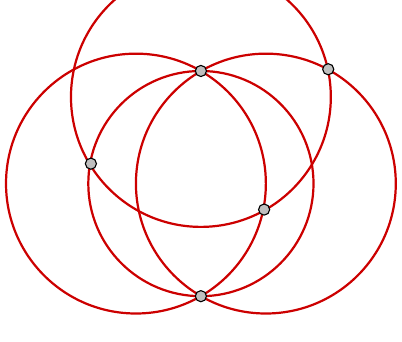
\begin{tikzpicture}[scale=1.1]
         \path[use as bounding box] (-2,-2) rectangle (2,1.3);
         \draw[thick,dark red] (-.75,-.5) circle (1.5);
         \draw[thick,dark red] (0,-.5) circle (1.3);
         \draw[thick,dark red] (.75,-.5) circle (1.5);
         \draw[thick,dark red] (0,.5) circle (1.5);
         \node[dot] at (0,.8) {};
         \node[dot] at (0,-1.8) {};
         \node[dot] at (1.47,.82) {};
         \node[dot] at (-1.27,-.27) {};
         \node[dot] at (.73,-.8) {};
    \end{tikzpicture}
\subcaption{Five dots in general position, and the four incident circles with one dot on either side}%$k=\ell=1$}
\label{fig: incidentexample}
\end{subfigure}
\begin{subfigure}[c]{0.45\linewidth}
\centering
    \[
    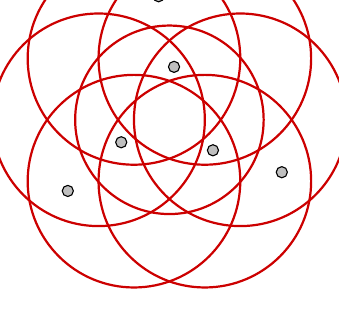
\begin{tikzpicture}[scale=.9]
         \path[use as bounding box] (-2,-2.4) rectangle (2,1.3);
        \draw[thick,dark red] (60:1) circle (1.5);
        \draw[thick,dark red] (120:1) circle (1.5);
        \draw[thick,dark red] (180:1) circle (1.5);
        \draw[thick,dark red] (240:1) circle (1.5);
        \draw[thick,dark red] (300:1) circle (1.5);
        \draw[thick,dark red] (0:1) circle (1.5);
        \draw[thick,dark red] (0,0) circle (1.33);
        \node[dot] at (90+5:1.75) {};
        \node[dot] at (210+5:1.75) {};
        \node[dot] at (330+5:1.75) {};
        \node[dot] at (30-5:-.75) {};
        \node[dot] at (150-5:-.75) {};
        \node[dot] at (270-5:-.75) {};
    \end{tikzpicture}
    \]
\subcaption{Six dots in general position, and seven avoidant circles with three dots on either side}%$k=\ell=3$}
\label{fig: avoidantexample}
\end{subfigure}
\caption{Incident and avoidant circles for two configurations of dots}
\label{fig: examples}
\end{figure}

%\vspace{-.4cm}

\section{Summary of results}

Consider a distinguished set of finitely many points in a plane or sphere, which we will call \textbf{dots}.
We say these dots are in \textbf{general position} if no four dots lie on a circle and (in the case of the plane) no three dots lie on a line.
By these assumptions, any three dots lie on a unique circle, which we call an \textbf{incident circle}, and this incident circle separates the remaining dots into two sets.%\footnote{In the case of the plane, these can be distinguished as the inside and the outside, but in the case of the sphere the two sides of a circle cannot be distinguished without an extra choice, such as an orientation.}

%Our first problem is the number of such circles which have fixed numbers of dots on the two sides. Remarkably, the answer does not depend on the configuration of the dots and is given by the following formula. 

Remarkably, if we count incident circles which have fixed numbers of dots on the two sides, the number does not depend on the configuration of the dots and is given by the following formula.

\begin{rethm}{A}\label{thm: incident}
%Let $n\geq4$. 
Given at least three dots in general position in the plane or sphere, the number of circles through three of the dots which separate the remaining dots into subsets of size $k$ and $\ell$ is
    \[
    \left\{
    \begin{array}{cc}
    2(k+1)(\ell+1) &\text{if $k\neq \ell$} \\
    (k+1)^2 &\text{if $k= \ell$} \\
    \end{array}
    \right\}
    \]
\end{rethm}

\begin{rem}
Note that we do not distinguish between the two sides of the circle, even in the plane. If we did, the analogous counts may depend on the configuration of the dots; see Example \ref{ex: interiorcircles}.
%For example, given any four dots in general position in the plane, all four incident circles separate the remaining dot into subsets of size 0 and 1. However, depending on the configuration of the dots, there might be 1, 2, or 3 incident circles with 0 dots on the inside and 1 dot on the outside.
\end{rem}

% \begin{figure}[h!tb]
% \centering
%     \begin{tikzpicture}[scale=1]
%          \path[use as bounding box] (-2,-2) rectangle (2,1.6);
%          \draw[thick,dark red] (-.75,-.5) circle (1.5);
%          \draw[thick,dark red] (0,-.5) circle (1.3);
%          \draw[thick,dark red] (.75,-.5) circle (1.5);
%          \draw[thick,dark red] (0,.5) circle (1.5);
%          \node[dot] at (0,.8) {};
%          \node[dot] at (0,-1.8) {};
%          \node[dot] at (1.47,.82) {};
%          \node[dot] at (-1.27,-.27) {};
%          \node[dot] at (.73,-.8) {};
%     \end{tikzpicture}
% \caption{Five dots in general position, and the four incident circles with $k=\ell=1$}
% \label{fig: incidentexample}
% \end{figure}

We also consider circles which pass through none of the dots, which we call \textbf{avoidant circles}. Of course, there are infinitely many such circles, but they only induce finitely many partitions of the dots. 
If we count such partitions with a fixed number of dots in the two parts, the number again does not depend on the configuration of the dots and is given by the following formula. 

\begin{rethm}{B}\label{thm: avoidant}
%Let $n\geq4$. 
Given at least three dots in general position in the plane or sphere, the number of partitions of the dots into non-empty subsets of size $k$ and $\ell$ which can be separated by a circle is
    \[
    \left\{
    \begin{array}{cc}
    2k \ell - k - \ell + 2 &\text{if $k\neq \ell$} \\
    k^2 - k + 1 &\text{if $k= \ell$} \\
    \end{array}
    \right\}
    \]
\end{rethm}

\noindent If we say two avoidant circles are \emph{equivalent} if they induce the same partition of the dots, then this theorem can be interpreted as counting avoidant circles up to equivalence.

% \begin{figure}[h!tb]
% \centering
%     \[
%     \begin{tikzpicture}[scale=1]
%         \draw[thick,dark red] (60:1) circle (1.5);
%         \draw[thick,dark red] (120:1) circle (1.5);
%         \draw[thick,dark red] (180:1) circle (1.5);
%         \draw[thick,dark red] (240:1) circle (1.5);
%         \draw[thick,dark red] (300:1) circle (1.5);
%         \draw[thick,dark red] (0:1) circle (1.5);
%         \draw[thick,dark red] (0,0) circle (1.33);
%         \node[dot] at (90+5:1.75) {};
%         \node[dot] at (210+5:1.75) {};
%         \node[dot] at (330+5:1.75) {};
%         \node[dot] at (30-5:-.75) {};
%         \node[dot] at (150-5:-.75) {};
%         \node[dot] at (270-5:-.75) {};
%     \end{tikzpicture}
%     \]

% \caption{Six dots in general position, and seven avoidant circles with $k=\ell=3$}
% \label{fig: avoidantexample}
% \end{figure}

Our primary tool in the latter theorem is the \emph{$k$th order Voronoi decomposition} of the sphere, which is the partition into regions based on which $k$-element subset of the dots is closest.
When $k=1$, this is the classical \emph{Voronoi decomposition} into regions based on which dot is the closest.

Regions in the $k$th Voronoi decomposition of the sphere are in bijection\footnote{Except when there are exactly $2k$-many dots, in which case the correspondence is 2-to-1.} with avoidant circles that have $k$-many dots on one side (up to equivalence). Theorem \ref{thm: avoidant} then reduces to a count of these regions, which may be deduced from Theorem \ref{thm: incident} and an Euler characteristic argument.

\begin{rem}
The analogous argument does not work in the plane, since the $k$th order Voronoi regions in the plane correspond to equivalence classes of avoidant circles with $k$-many points in their interior, and the number of such circles can depend on the configuration of the dots.
%
Theorem \ref{thm: avoidant} is still valid in the plane, but we must deduce it from the spherical case via \emph{stereographic projection}.
\end{rem}

We also consider how the $k$th order Voronoi decomposition of the sphere (and thus the incident and avoidant circles) changes as the configuration of dots moves around. If we color the vertices of this decomposition black and white (based on the number of dots on each side of the corresponding incident circle), we can regard the $k$th order Voronoi decomposition as a bicolored graph in the sphere. 
%
%The vertices of this decomposition naturally come in two flavors (based on the number of dots on each side of the corresponding incident circle), and so we can regard the $k$th order Voronoi decomposition as a bicolored graph in the sphere.
%
As long as the deformation of the dots is `general enough', we show this bicolored graph will change by a sequence of the three local `moves' appearing in Figure \ref{fig: postnikovmoves} (Lemma \ref{lemma: move}). 

\begin{figure}[h!t]
\[
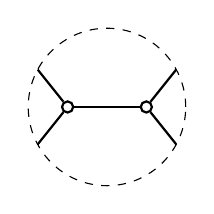
\begin{tikzpicture}[scale=.5,baseline=(a.base)]
        \draw[dashed] (0,0) circle (2);
        \clip (0,0) circle (2);
        \node[dot,thick,fill=white] (1) at (180:1) {};
        \node[dot,thick,fill=white] (3) at (0:1) {};

        \draw[thick] (1) to (3);
        \draw[thick] (1) to (-5,5);
        \draw[thick] (1) to (-5,-5);
        \draw[thick] (3) to (5,5);
        \draw[thick] (3) to (5,-5);

        \node[opacity=0] (a) at (0,0) {$a$};
\end{tikzpicture}
\leftrightarrow
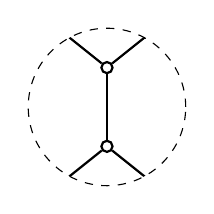
\begin{tikzpicture}[scale=.5,baseline=(a.base)]
        \draw[dashed] (0,0) circle (2);
        \clip (0,0) circle (2);
        \node[dot,thick,fill=white] (2) at (90:1) {};
        \node[dot,thick,fill=white] (4) at (270:1) {};

        \draw[thick] (2) to (4);
        \draw[thick] (2) to (-5,5);
        \draw[thick] (4) to (-5,-5);
        \draw[thick] (2) to (5,5);
        \draw[thick] (4) to (5,-5);

        \node[opacity=0] (a) at (0,0) {$a$};
\end{tikzpicture}
\hspace{.75cm}
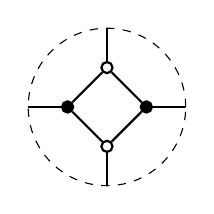
\begin{tikzpicture}[scale=.5,baseline=(a.base)]
        \draw[dashed] (0,0) circle (2);
        \clip (0,0) circle (2);
        \node[dot,thick,fill=black] (1) at (180:1) {};
        \node[dot,thick,fill=white] (2) at (90:1) {};
        \node[dot,thick,fill=black] (3) at (0:1) {};
        \node[dot,thick,fill=white] (4) at (270:1) {};

        \draw[thick] (1) to (2);
        \draw[thick] (2) to (3);
        \draw[thick] (3) to (4);
        \draw[thick] (4) to (1);
        \draw[thick] (1) to (-5,0);
        \draw[thick] (2) to (0,5);
        \draw[thick] (3) to (5,0);
        \draw[thick] (4) to (0,-5);

        \node[opacity=0] (a) at (0,0) {$a$};
\end{tikzpicture}
\leftrightarrow
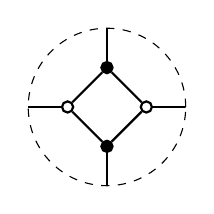
\begin{tikzpicture}[scale=.5,baseline=(a.base)]
        \draw[dashed] (0,0) circle (2);
        \clip (0,0) circle (2);
        \node[dot,thick,fill=white] (1) at (180:1) {};
        \node[dot,thick,fill=black] (2) at (90:1) {};
        \node[dot,thick,fill=white] (3) at (0:1) {};
        \node[dot,thick,fill=black] (4) at (270:1) {};

        \draw[thick] (1) to (2);
        \draw[thick] (2) to (3);
        \draw[thick] (3) to (4);
        \draw[thick] (4) to (1);
        \draw[thick] (1) to (-5,0);
        \draw[thick] (2) to (0,5);
        \draw[thick] (3) to (5,0);
        \draw[thick] (4) to (0,-5);

        \node[opacity=0] (a) at (0,0) {$a$};
\end{tikzpicture}
\hspace{.75cm}
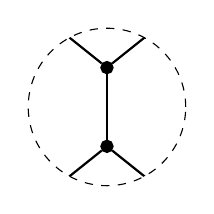
\begin{tikzpicture}[scale=.5,baseline=(a.base)]
        \draw[dashed] (0,0) circle (2);
        \clip (0,0) circle (2);
        \node[dot,thick,fill=black] (2) at (90:1) {};
       \node[dot,thick,fill=black] (4) at (270:1) {};

        \draw[thick] (2) to (4);
        \draw[thick] (2) to (-5,5);
        \draw[thick] (4) to (-5,-5);
        \draw[thick] (2) to (5,5);
        \draw[thick] (4) to (5,-5);

        \node[opacity=0] (a) at (0,0) {$a$};
\end{tikzpicture}
\leftrightarrow
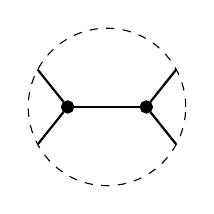
\begin{tikzpicture}[scale=.5,baseline=(a.base)]
        \draw[dashed] (0,0) circle (2);
        \clip (0,0) circle (2);
        \node[dot,thick,fill=black] (1) at (180:1) {};
        \node[dot,thick,fill=black] (3) at (0:1) {};

        \draw[thick] (1) to (3);
        \draw[thick] (1) to (-5,5);
        \draw[thick] (1) to (-5,-5);
        \draw[thick] (3) to (5,5);
        \draw[thick] (3) to (5,-5);

        \node[opacity=0] (a) at (0,0) {$a$};
\end{tikzpicture}
\]
\caption{Three local moves between bicolored graphs in the sphere}
\label{fig: postnikovmoves}
\end{figure}

Since any two configurations of the same number of dots can be connected by such a deformation, we deduce the following.


% If a continuous family of dots remains in general position at all times, then the underlying graph of the $k$th order Voronoi decomposition does not change.
% It is therefore more interesting to consider continuous families of dots that can be in \emph{semigeneral position} (i.e.~fail to be in general position in simplest way possible way) finitely many times. We show that, along such a family, the $k$th order Voronoi decomposition will change via a sequence of three local `moves' (Figure \ref{???}). 

% FIGURE

% Since any two configurations of the same number of dots in the sphere can be related by such a family, we arrive at the following observation.

%These same moves appeared in Postnikov's seminal work on bicolored planar graphs \cite{???}; two graphs are called \emph{move-equivalent} if they are related by a sequence of the local moves in Figure \ref{???}. Move-equivalent planar graphs have many features in common, for example, they determine isomorphic cluster algebras via the construction in \cite{???}.

\begin{rethm}{C}\label{thm: move equiv}
Let $0<k<n>3$. The $k$th order Voronoi decompositions of any two sets of $n$-many dots in general position in the sphere may be related by a sequence of the local moves in Figure \ref{fig: postnikovmoves}.
%Any two sets of the same number of dots in general position in the sphere have $k$th order Voronoi decompositions that are 
%\emph{move-equivalent}. %Therefore, they determine isomorphic cluster algebras.
\end{rethm}



These same moves appeared in Postnikov's seminal work on planar bicolored graphs \cite{Pos}. %, where graphs related by a sequence of these moves were called \emph{move-equivalent}.
%if they are related by a sequence of the local moves in Figure \ref{???}. 
Graphs related by these moves have many features in common, for example, they determine isomorphic cluster algebras. % via the construction in \cite{???}. 
%We sketch the connection to cluster algebras in Section \ref{???}.
%
The theorem implies that the $k$th order Voronoi decompositions of any two configurations of $n$-many dots in the sphere determine isomorphic cluster algebras. Cluster algebras constructed this way include several important examples, such as the \emph{Markov cluster algebra} and the \emph{$X_7$ cluster algebra}; preliminary results are discussed briefly in Section \ref{sec: future}.%We outline the expected structure of these cluster algebras in Section \ref{???}.

\begin{rem}
Versions of these counting problems and the resulting formulas have been considered in many previous works, such as the $k=\ell$ version of Theorem \ref{thm: incident} appearing in \cite{Ard04}. Most notably, Theorems \ref{thm: incident} and \ref{thm: avoidant} were proven in full generality in \cite{CHP22}. In that paper, the counts are deduced by constructing spherical Voronoi decompositions from gluing together pairs of planar Voronoi decompositions and then using a symmetry in planar Voronoi decompositions observed in \cite{Lin03} (see Appendix \ref{appendix}).
%the results are derived from a formula in \cite{Lin03} for sums of vertices in pairs of higher order Voronoi decompositions of the plane. 
Our argument suggests that the more natural derivation may be the other direction, by first counting the numbers of cells in spherical higher order Voronoi decompositions and then using the gluing map in \cite{CHP22} to deduce the symmetry in \cite{Lin03}.
\end{rem}

% MENTION PREVIOUS WORKS
% \nocite{Ard04}
% \nocite{CHP22}
% \nocite{Lin03}

%In Section \ref{???}, we sketch this connection more in depth. 

\subsection*{Acknowledgements}

The authors are most grateful for the organizers of the Early Career Conference in Combinatorics held at the University of Illinois Urbana-Champaign in June 2024, where a version of this problem was presented in an open problem session, leading to this collaboration.

\section{Dots in the sphere or plane}

Throughout this note, we let $D$ denote a finite set of points, which we call \textbf{dots}, which may be in either a plane $P$ or a sphere $S$. We say the configuration of dots $D$ is in \textbf{general position} if
\begin{itemize}
    \item no four dots lie on a circle, and
    \item (in the case of the plane) no three dots lie on a line.
\end{itemize}
% Throughout this note, we consider a distinguished set of points $D$, which we call \textbf{dots}, in a sphere $S$ or plane $P$. 
% We say these dots are in \textbf{general position} if no four dots lie on a circle and (in the case of the plane $P$) no three dots lie on a line.
%Since every circle in $S^2$ can be realized as the intersection with a plane in $\mathbb{R}^3$, an equivalent condition is that no four dots lie on a plane in $\mathbb{R}^3$.
%Generally speaking, most of our lemmas and proofs will be in the sphere; however, because the ultimate results are both valid and interesting in the plane 

We can translate between configurations of dots in the plane and in the sphere via a \emph{stereographic projection} map.
%Most of our results will be equally valid in the sphere and the plane, because we can translate between the two via \emph{stereographic projection}. 
To define such a map, choose an embedding of both the sphere $S$ and the plane $P$ in 3-dimensional space, and choose a {point} $p_\infty \in S$ whose tangent plane is parallel to $P$ but not equal to $P$.\footnote{For example, one may always choose $p_\infty$ to be the furthest point on $S$ from $P$.}
%
The corresponding \textbf{stereographic projection} of a point $p$ in $S\smallsetminus p_\infty$ is defined to be the unique point $\pi(p)$ on $P$ which lies on the line connecting $p$ and $p_\infty$.% (Figure \ref{fig: stereo}).

% %
% For each point $p\in S^2$ other than $p_\infty$, there is a line through $p$ and $p_\infty$, which intersects the plane $P$ at a unique point $\pi(p)$. Stereographic projection is then the map $\pi:S^2\smallsetminus p_\infty \rightarrow P$.

% Consider a finite set of points in the plane, which we will call \textbf{dots}. We say these dots are in \textbf{general position} if no three dots lie on a line and no four dots lie on a circle.\footnote{The first condition is one of convenience; most of what follows remains true without it, provided we expand our definition of `circle' to include lines.}

% It will be useful to move back and forth between the plane and the sphere via \textbf{stereographic projection}. 

% Consider a plane $P$ and a sphere $S$ in $\mathbb{R}^3$, and choose a point $p_\infty$ on the sphere $S$ whose tangent plane is parallel to the given plane $P$. For each point in $p\in P$, there is a 
\begin{figure}[h!t]
    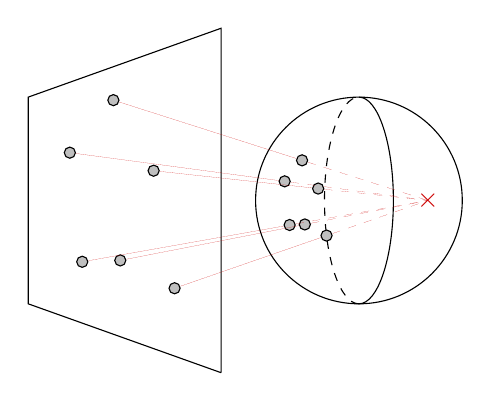
\begin{tikzpicture}[scale=1.75,rotate=90]
        \node[dot] (d1) at (-.445,.258) {};
        \node[dot] (d2) at (.347,.348) {};
        \node[dot] (d3) at (.728,.032) {};
        \node[dot] (d4) at (.216,-.26) {};
        \node[dot] (d5) at (-.435,-.018) {};
        \node[dot] (d6) at (-.637,-.412) {};

        \draw (-1.25,-.75) to (1.25,-.75) to (.75,.65) to (-.75,.65) to (-1.25,-.75);

        \begin{scope}[yshift=-1.75cm]
            \draw (0,0) circle (.75);
    
            \draw (-.75,0) arc [start angle=180, end angle=360, x radius=.75, y radius=.25];
            \draw[dashed] (-.75,0) arc [start angle=180, end angle=0, x radius=.75, y radius=.25];
    
            \coordinate (point) at (0,-.5);
            \node[dark red] at (point) {$\times$};
        \end{scope}

        \def\ta{.4};
        \def\tb{.4};
        \def\tc{.4};
        \def\td{.4};
        \def\te{.4};
        \def\tf{.4};

        \node[dot] (p1) at ($\ta*(d1)+{1-\ta}*(point)$) {};
        \node[dot] (p2) at ($\tb*(d2)+{1-\tb}*(point)$) {};
        \node[dot] (p3) at ($\tc*(d3)+{1-\tc}*(point)$) {};
        \node[dot] (p4) at ($\td*(d4)+{1-\td}*(point)$) {};
        \node[dot] (p5) at ($\te*(d5)+{1-\te}*(point)$) {};
        \node[dot] (p6) at ($\tf*(d6)+{1-\tf}*(point)$) {};

        \draw[projection line] (d1) to (p1);
        \draw[projection line] (d2) to (p2);
        \draw[projection line] (d3) to (p3);
        \draw[projection line] (d4) to (p4);
        \draw[projection line] (d5) to (p5);
        \draw[projection line] (d6) to (p6);
        \draw[projection line,dashed] (p1) to (point);
        \draw[projection line,dashed] (p2) to (point);
        \draw[projection line,dashed] (p3) to (point);
        \draw[projection line,dashed] (p4) to (point);
        \draw[projection line,dashed] (p5) to (point);
        \draw[projection line,dashed] (p6) to (point);
        
    
        % \draw[blue] (-.104,-.085) circle (.5544);
        % \draw[blue] (.087,-.116) circle (.5911);
        % \draw[blue] (.128,.307) circle (.6126);
        % \draw[blue] (.17,-.433) circle (.7672);
        % \draw[blue] (-.102,.28) circle (.5404);
        % \draw[blue] (.41,.087) circle (.6245);
        % \draw[blue] (-.01,-.387) circle (.7027);
    \end{tikzpicture}
\caption{Stereographic projection of 6 dots}
\label{fig: stereo}
\end{figure}

Stereographic projection defines a homeomorphism $\pi$ between the punctured sphere $S\smallsetminus p_\infty$ and the plane $P$ which has many nice properties; e.g.~stereographic projection induces bijections
\[
\begin{aligned}
\{\text{circles in $S$ which contain $p_\infty$}\} &\xrightarrow{\sim} \{\text{lines in $P$}\}
\\
\{\text{circles in $S$ which do not contain $p_\infty$}\} &\xrightarrow{\sim} \{\text{circles in $P$}\}
\end{aligned}
\]
As an immediate consequence, configurations of dots in general position in one space can be translated to configurations of dots in general position in the other space.
\begin{prop}
A configuration of dots $D$ in the sphere $S$ is in general position if and only if there is a stereographic projection $\pi:S\smallsetminus p_\infty\rightarrow P$ such that $\pi(D)$ is in general position in the plane $P$.
\end{prop}

As we will see, the numbers of incident and avoidant circles we want to count are also preserved by stereographic projection.
As a consequence, we can work primarily in one surface (usually, the sphere $S$) but deduce results in both surfaces.

% \begin{proof}
% Choose a $p_\infty$ in $S$ which is not on any incident circle through three dots in $D$. 
% \end{proof}

\begin{warn}
Even when $\pi$ sends a circle to a circle, it does not preserve the centers of those circles.
%While stereographic projection sends circles in $S$ to circles and lines in $P$, it does not preserve the centers of those circles. 
Similarly, it does not send geodesics in $S$ (i.e.~great circles) to geodesics in $P$ (i.e.~lines). This leads to a qualitative difference between the \emph{higher order Voronoi decompositions} (see Appendix \ref{appendix}).
\end{warn}

% \begin{warn}
% Stereographic projection does not send the center of a circle in $S^2$ to the center of the projected circle in $P$.
% \end{warn}

% Therefore, a circle in the sphere $S^2$ which separates the dots into sets of size $k$ and $\ell$ will project to a circle (or line) in the plane $P$ which separates the projected dots into sets of size $k$ and $\ell$. In this way, our counts of such circles will be equally valid in the sphere and the plane.


% this defines a pair of bijections
% \[
% \begin{aligned}
% \{\text{circles in $S^2$ disjoint from $p_\infty$}\}
% &\xrightarrow{\pi}
% \{\text{circles in $P$}\} 
% \\
% \{\text{circles in $S^2$ passing through $p_\infty$}\}
% &\xrightarrow{\pi}
% \{\text{lines in $P$}\}
% \end{aligned}
% \]

% \begin{thm}
% Stereographic projection defines a 
% \end{thm}

% It will be convenient to consider \textbf{oriented} circles in the sphere or plane. The orientation allows us to distinguish between the \textbf{left} and \textbf{right} sides of the circle. 



%\subsection{Separating dots with incident circles}


%In this paper, we count various ways to separate these dots into circles. 

%Consider a finite set of points in the plane, which we will call \textbf{dots} to distinguish them from other points in the plane. We say these dots are in \textbf{general position} if no three dots lie on a line and no four dots lie on a circle.\footnote{The first condition is one of convenience; most of what follows remains true without it, provided we expand our definition of `circle' to include lines.}

%Count the number of ways to use a circle to separate the dots into partitions of a fixed size.

%\subsection{Incident circles}

\section{Counting incident circles}

Let $D$ be a finite set of dots in general position in the plane $P$ or sphere $S$. 
Any three dots in $D$ lie on a unique \textbf{incident circle},\footnote{
The circle through three points in the plane is sometimes called the \emph{circumcircle}, particularly when the three points are the vertices of a triangle. We avoid this language, as we are not interested in the triangle spanned by the dots.}
and this circle separates the remaining dots into two sets. 
%While we are primarily interested in unoriented incident circles, it will also be useful to consider \textbf{oriented incident circles}, since this lets use distinguish between 
%If we choose an orientation of the circle, we can
%
% In the plane $P$, we can distinguish these two sets as the `inside' and the `outside', but there is no analogous distinction in the sphere $S$ (also, making this distinction leads to a poorly behaved counting problem, see Example \ref{???}). 
% However, if we \textbf{orient} the circle, then we can distinguish these two sets as the \textbf{left side} and the \textbf{right side}, which makes sense in both $P$ and $S$ (and leads to a well-behaved counting problem; see Proposition \ref{prop: orientedincident}).
%
% %Consider a finite set of dots in general position in the sphere $S^2$.
% An \textbf{incident circle (through $D$)} is a circle which passes through three of the dots.
% %such a circle is uniquely determined by the three dots.%
% %Any three dots determines a unique circle through those dots, which we call an \textbf{incident circle}. 
% Because the dots are in general position, an incident circle is determined by the three dots it passes through, and it separates the remaining dots into two sets. If the incident circle is oriented, we can distinguish these two sets as the \textbf{left side} and the \textbf{right side}.
%
We are interested in counting incident circles %(both oriented and unoriented) 
with fixed numbers of dots on either side. We start with the following, which will form the base case of our induction.

\begin{prop}\label{prop: incident0}
Let $n\geq4$. Given $n$-many dots $D$ in general position in the sphere $S$, there are $(2n-4)$-many incident circles with no dots on one side.
\end{prop}

\begin{proof}
%Let $D\subset S^2$ denote the set of dots, and l
Choose an embedding of the sphere $S$ in $\mathbb{R}^3$, and let $H$ denote the convex hull of $D$ as a subset of $\mathbb{R}^3$. 
Since the dots are in general position, at most 3 dots can lie on any plane in $\mathbb{R}^3$, and so each face of the convex hull $H$ must be a triangle. Since each edge of $H$ lies in two faces and each triangle has three edges,
\[ 
2(\text{$\#$ of edges in $H$})
=
3(\text{$\#$ of faces in $H$})
\]
The vertices of $H$ are the $n$-many dots $D$, so the Euler characteristic of $H$ tells us that
\[
2 = n - (\text{$\#$ of edges in $H$}) + (\text{$\#$ of faces in $H$}) %= n - \frac{1}{2} (\text{$\#$ of faces in $H$})
\]
Solving the previous two equations tells us that the number of faces of $H$ must be $2n-4$.

Given three dots $\{a,b,c\}\subset D$, the incident circle through those dots is the intersection of the affine plane through $\{a,b,c\}$ in $\mathbb{R}^3$ with the sphere $S$. Therefore, the incident circle through $\{a,b,c\}$ has no dots on one side if and only if the plane through $\{a,b,c\}$ bounds a half-space in $\mathbb{R}^3$ which contains the convex hull $H$; equivalently, $\{a,b,c\}$ lie on a face of the convex hull $H$. Since each face of $H$ is a triangle, the face uniquely determines the three dots $\{a,b,c\}$. Therefore, we have a bijection between incident circles with no dots on one side and faces in the convex hull $H$.
\end{proof}

% \begin{lemma}

% \end{lemma}

For the next proposition, we want to distinguish between the two sides of an incident circle. We can do this by choosing an orientation, so  we can distinguish the \textbf{left side} and the \textbf{right side}.

\begin{prop}\label{prop: orientedincident}
Let $n\geq3$ and $0\leq k \leq n-3$. Given $n$-many dots $D$ in general position in the sphere $S$, there are 
\[I_{k,n} := 2(k+1)(n-k-2)\]
oriented incident circles with $k$-many dots on their left side (and thus $n-k-3$ dots on the right).
\end{prop}

\begin{proof}
If $n=3$, then $k=0$. Since the unique incident circle through the three dots has $2=I_{0,3}$ orientations, the theorem holds in this case. %In what follows, assume $n\geq4$.% and so Proposition \ref{prop: incident0} applies.

We prove the $n\geq4$ case by induction on $k$. 
If $k=0$, then Proposition \ref{prop: incident0} implies there are $(2n-4)$-many incident circles with no dots on one side. Since $n\geq4$, the other side must have at least 1 dot and there is a unique orientation of each such circle which has no dots on the left side. Thus, there are $I_{0,n}=2\cdot 1\cdot(n-2)$-many oriented incident circles with $0$ dots on their left side.

Next, assume the proposition holds for $k-1$, and consider a configuration $D$ of $n$-many dots in general position in $S$. 
There are $n$-many ways to choose a dot $d\in D$ to delete; by assumption, there are then $I_{k-1,n-1}$-many ways to choose an oriented incident circle through three of the remaining $(n-1)$-many dots which has $(k-1)$-many dots on its left side. 
Therefore, there are
\[
n \cdot I_{k-1,n-1} = 2nk(n-k-2)
\]
ways to delete a dot and then choose an oriented incident circle with $k-1$ dots on its left side.

Alternatively, we could first choose the circle, then choose the dot to delete. This can be done in two disjoint ways.
    \begin{itemize}
        \item First choose an oriented incident circle with $(k-1)$-many dots on its left side, then choose a dot on that circle's right side to delete. By assumption, the number of ways to do this is
        \[
        I_{k-1,n}\cdot (n-k-2) = 2k(n-k-1)(n-k-2)
        \]
        \item First choose an oriented incident circle with $k$-many dots on its left side, then choose a dot on that circle's left side to delete. The number of ways to do this is
        \[
        (\text{$\#$ of oriented incident circles of $D$ with $k$-many dots on their left side})\cdot k
        \]
    \end{itemize}
Since this constructs the same set as before, the sum of these two counts is equal to $nI_{k-1,n-1}$. Solving this equality for the desired number of circles,
\[
% 2nk(n-k-3)
% =
% 2k(n-k-2)(n-k-3)
% +
(\text{$\#$ of oriented incident circles of $D$ with $k$-many dots on their left side})
%= 2n(n-k-3) - 2(n-k-1)(n-k-3)
=2(k+1)(n-k-2)%=:I_{k,n}
\]
This completes the induction.
\end{proof}

\begin{rem}
The heart of the proof is a double counting argument which can be summarized as
\[ nI_{k-1,n-1} = (n-k-2)I_{k-1,n} + kI_{k,n} 
\qedhere
\]
%However, 
\end{rem}

% The computation to check. Let $\mathbb{I}_{k,n}$ denote the number of oriented incident circles through $n$-many dots in general position with $k$-many dots on their left side. Then the above double counting argument shows that 
% \[
% n\mathbb{I}_{k-1,n-1} = (n-k-2)\mathbb{I}_{k-1,n} + k\mathbb{I}_{k,n} 
% \]
% If we assume for induction that
% \[
% \begin{aligned}
% \mathbb{I}_{k-1,n} &= 2k(n-k-1) \\
% \mathbb{I}_{k-1,n-1}  &= 2k(n-k-2)
% \end{aligned}
% \]
% Combined with the double counting identity,
% \[
% \begin{aligned}
% k\mathbb{I}_{k,n} 
% &= n\mathbb{I}_{k-1,n-1} - (n-k-2)\mathbb{I}_{k-1,n} \\
% &= n(2k(n-k-2)) - (n-k-2)(2k(n-k-1)) \\
% &= 2k(n -(n-k-1))(n-k-2) = 2k(k+1)(n-k-2)
% \end{aligned}
% \]
% Dividing by $k$ confirms the asserted identity.

It is now a simple matter to adapt this to count unoriented incident circles.

\begin{rethm}{\ref{thm: incident}}
%Let $n\geq4$. 
Given at least three dots in general position in the plane or sphere, the number of circles through three of the dots which separate the remaining dots into subsets of size $k$ and $\ell$ is
    \[
    \left\{
    \begin{array}{cc}
    2(k+1)(\ell+1) &\text{if $k\neq \ell$} \\
    (k+1)^2 &\text{if $k= \ell$} \\
    \end{array}
    \right\}
    \]
\end{rethm}

\begin{proof}
Since exactly 3 dots lie on an incident circle, there must be $n:=k+\ell+3$ dots. %If $n=3$, then $k=\ell=0$, and the unique incident circle through the three dots matches the $(k+1)^2$ in the formula. For the remainder of the proof, assume $n\geq4$ and so Proposition \ref{prop: orientedincident} applies.

If $k\neq \ell$, then such an incident circle has a unique orientation with $k$-many dots on its left side. By Proposition \ref{prop: orientedincident}, the number of such oriented incident circles in the sphere is 
\[
2(k+1)(n-k-2) = 2(k+1)(\ell+1)
\]

If $k=\ell$, then then such an incident circle has two orientations with $k$-many dots on the left side. By Proposition \ref{prop: orientedincident}, the number of such oriented incident circles in the sphere is 
\[
2(k+1)(n-k-2) = 2(k+1)(\ell+1)= 2(k+1)^2
\]
Dividing by $2$, the number of unoriented incident circles with $k$-many dots on one side is $(k+1)^2$.

This proves the theorem for dots in the sphere $S$.
Since incident circles and the sets of dots on either side are preserved by stereographic projection, the theorem holds for dots in the plane $P$.
\end{proof}

\begin{ex}\label{ex: interiorcircles}
Given a configuration of dots in the plane, it may seem more natural to count incident circles with a fixed number of dots on the inside (rather than on either of the sides). However, the number of such circles can depend on the specific configuration.

To see this, consider the two configurations of 4 dots in general position in the plane given in Figure \ref{fig: fourdots}. Each configuration admits $\binom{4}{3}=4$ incident circles. In Figure \ref{fig: fourdotsonecircle}, only one of those circles has a dot on the inside, while, in Figure \ref{fig: fourdotstwocircles}, two of those circles have a dot on the inside.

\begin{figure}[h!tb]
\captionsetup[subfigure]{justification=centering}
\centering
\begin{subfigure}[c]{0.45\linewidth}
\centering
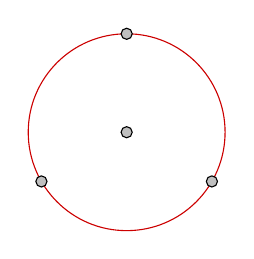
\begin{tikzpicture}[inner sep=0.5mm,scale=1.25,auto]
	\draw[dark red] (0,0) circle (1);
	\node[dot] (0) at (0,0) [circle,draw] {};
	\node[dot] (1) at (90:1) [circle,draw] {};
	\node[dot] (2) at (-30:1) [circle,draw] {};
	\node[dot] (3) at (210:1) [circle,draw] {};
\end{tikzpicture}
\subcaption{A configuration of four dots admitting a unique incident circle with one interior dot}
\label{fig: fourdotsonecircle}
\end{subfigure}
\begin{subfigure}[c]{0.45\linewidth}
\centering
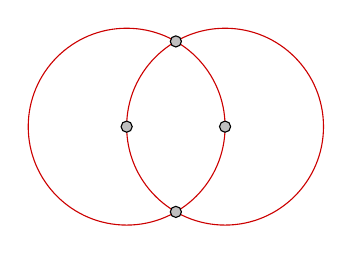
\begin{tikzpicture}[inner sep=0.5mm,scale=1.25,auto]
	\draw[dark red] (.5,0) circle (1);
	\draw[dark red] (-.5,0) circle (1);
	\node[dot] (0) at (.5,0) [circle,draw] {};
	\node[dot] (1) at (-.5,0) [circle,draw] {};
	\node[dot] (2) at (0,.866) [circle,draw] {};
	\node[dot] (3) at (0,-.866) [circle,draw] {};
\end{tikzpicture}
\subcaption{A configuration of four dots admitting two incident circles with one interior dot}
\label{fig: fourdotstwocircles}
\end{subfigure}
\caption{Two configurations of four dots in general position in the plane}
\label{fig: fourdots}
\end{figure}

Note that the three incident circles not pictured in 
Figure \ref{fig: fourdotsonecircle} and the two incident circles not pictured in Figure \ref{fig: fourdotstwocircles} each have 0 dots in the inside and 1 dot on the outside.
Therefore, in both configurations, all four incident circles separate the remaining dot(s) into subsets of sizes $k=1$ and $\ell=0$, matching the formula in Theorem \ref{thm: incident}.
\end{ex}



% \begin{tikzpicture}[inner sep=0.5mm,scale=1.25,auto]
% 	\draw[dark red] (.5,0) circle (1);
% 	\draw[dark red] (-.5,0) circle (1);
% 	\node[dot] (0) at (.5,0) [circle,draw] {};
% 	\node[dot] (1) at (-.5,0) [circle,draw] {};
% 	\node[dot] (2) at (0,.866) [circle,draw] {};
% 	\node[dot] (3) at (0,-.866) [circle,draw] {};
% 	\node[dot] (4) at (0,.25) [circle,draw] {};
% \end{tikzpicture}

% \subsection{Convex hulls}

% \begin{lemma}
% Let $n\geq 4$, and consider $n$-many dots $D$ in general position in the sphere $S^2$. Given $a,b,c\in D$, the incident circle through $a,b,c$ has no dots on one side iff the 

% A triple of dots lies on an incident circle with no dots on one side if and only if th
% \end{lemma}

%\newpage

\section{Higher order Voronoi decompositions}\label{sec: higher Voronoi}

\def\dis{\operatorname{dist}}

Our primary tool for counting avoidant circles will be the \emph{$k$-th order Voronoi decomposition} of the sphere determined by a configuration of dots $D$. Roughly speaking, this decomposes the sphere into regions based on which $k$-element subset of the dots is the closest to a given point.\footnote{
Higher order Voronoi decompositions may also be defined in the plane (or any metric space), but they are not as nicely behaved as that of the sphere. In particular, the number of vertices, edges, and faces may depend on the configuration. See Appendix \ref{appendix} for a discussion of the planar case and the relation to the spherical case.
}  A survey of results relating to higher order Voronoi diagrams can be found in Edelsbrunner’s book on algorithms in combinatorial geometry \cite{EdelsbrunnerBook}, though our discussion here assumes no prior knowledge.


% \begin{defn}
% Let $D$ be a finite set of dots in $X$. %the sphere or plane, denoted $X$.
% The \textbf{$k$th order Voronoi decomposition} of $X$ determined by $D$ consists of \textbf{Voronoi cells} of the form
% % \[
% % R_{D_0} = \{ p\in S\text{ or } P \mid D_-(p) \supseteq D_0 \}
% % \]
% \[
% R_{K} = \{ p\in X \text{ such that, for all $d\in K$ and $d'\in D\smallsetminus K$, }\dis(p,d) < \dis(p,d') \}
% \]
% where $K$ runs over all $k$-element subsets of $D$.
% \end{defn}

%However, we will use a more delicate construction to 

% \begin{infdefn}
% The \emph{$k$th order Voronoi decomposition of $S$ or $P$ determined by the dots $D$ is the decomp
% \end{infdefn}


% Given a point $p\in S^2$, define a pair of sets
% \[
% \begin{aligned}
% D_-(p)&:= \{d\in D \mid \dis(p,d) \leq \dis(p,d_k) \} \\
% %\text{ and }
% D_+(p)&:= \{d\in D \mid \dis(p,d) \geq \dis(p,d_{k+1}) \} \\
% \end{aligned}
% \]
% where we 

%Fix a set of $n$-many dots $D$ in the sphere $S$, and a positive integer $k< n$. 

%To make this specific, let us fix integers $0<k<n>3$ for the rest of this section. 

% Given any two points $p,q$ in the sphere $S$, let $\dis(p,q)$ 
% %Let $D$ be a configuration of $n$-many dots in the sphere $S$, and let $\dis(p,q)$ 
% denote the geodesic distance between any two points $p,q\in S$.

Given a configuration of dots $D$ in the sphere $S$ and an arbitrary point $p\in S$, 
index the dots $d_1,d_2,\dotsc,d_n$ in $D$ by weakly increasing distance from $p$; that is,
\[
\dis(p,d_1)\leq \dis(p,d_2) \leq \dotsb \leq \dis(p,d_n) 
\]
where $\dis(p,q)$ denotes the geodesic distance between any two points $p,q\in S$.

Fix an integer $0<k<n$. For each point $p\in S$, we use the temporary indexing above to define a pair of sets (which ultimately do not depend on the choice of indexing)
%We use this indexing and a choice of integer $0<k<n$ to define a pair of sets% (which do not depend on the choice of indexing):
\[
\begin{aligned}
D_{-}(p)&:= \{d\in D \mid \dis(p,d) \leq \dis(p,d_k) \} \\
%\text{ and }
D_{+}(p)&:= \{d\in D \mid \dis(p,d) \geq \dis(p,d_{k+1}) \} \\
\end{aligned}
\]
%Note that these sets do not depend on the choice of indexing of $D$.
Informally, $D_{-}(p)$ is the set of dots that are at worst tied for $k$-closest to $p$, and $D_{+}(p)$ is the set of dots that are at best tied for $(k+1)$-closest to $p$.
While these two sets are often disjoint, they will overlap whenever there is a tie between the $k$th closest and the $(k+1)$-closest dots to $p$.

\begin{defn}
Let $0<k<n>3$ and let $D$ be a set of $n$-many dots in the sphere $S$. A \textbf{(closed) $k$th-order Voronoi stratum} is a subset $V\subset S$ of the form 
% For each point $p\in X$, the \textbf{(closed) Voronoi stratum} defined by $p$ is the subset of $X$ defined by
\[
\{ q\in S \text{ such that $D_-(p)\subseteq D_-(q)$ and $D_+(p)\subseteq D_+(q)$}\}
\]
for some point $p\in S$. The $k$th order Voronoi strata collectively form the \textbf{$k$th order Voronoi decomposition} of $S$ determined by $D$.
\end{defn}

%Two points $p,q\in S$ define the same Voronoi stratum

While many different points $p\in S$ may determine the same $k$th order Voronoi stratum, each $k$th order Voronoi stratum $V$ is uniquely determined by the pair of subsets (for any $p$ which defines $V$)
\begin{equation}\label{eq: Voronoisets}
D_-(V) := D_-(p)
\text{ and }
D_+(V) := D_+(p).
\end{equation}

The possible shapes of these strata are given as follows.

\begin{prop}\label{prop: stratumtypes}
Let $0<k<n>3$ and let $D$ be a configuration of $n$-many dots in general position in $S$. Then every $k$th order Voronoi stratum $V$ must be one of the following.
\begin{enumerate}
    \item A spherical polygon.
    \item A great circular arc.
    \item A single point.
\end{enumerate}
The cases are characterized by $D_-(V)\cap D_+(V)$ consisting of $0$, $2$, or $3$ dots, respectively.
%Furthermore, the three cases correspond to $|D_=(V)|=3$, $|D_=(V)|=2$, and $|D_=(V)|=0$.
\end{prop}

\noindent We refer to these three types of strata as \textbf{regions}, \textbf{edges}, and \textbf{vertices} in the $k$th order Voronoi decomposition, respectively. 



\begin{proof}
%Let $V$ be a Voronoi stratum, and let $D_-(V)$ and $D_+(V)$ be the subsets of $D$ defined by \eqref{eq: Voronoisets}. 
Letting $D_-(V)$ and $D_+(V)$ be as in \eqref{eq: Voronoisets}, the definition of $V$ can be reformulated as follows.
\[
\begin{aligned}
V 
&= \{ q\in S \text{ such that $D_-(V)\subseteq D_-(q)$ and $D_+(V)\subseteq D_+(q)$}\}
\\
&= \{ q\in S  \text{ such that, for all $d_-\in D_-(V), d_+\in D_+(V)$, $\dis(q,d_-)\leq \dis(q,d_+)$}\}
\\
&= 
\bigcap_{d_-\in D_-(V)}~ \bigcap_{d_+\in D_+(V)}
\{ q\in S  \text{ such that $\dis(q,d_-)\leq \dis(q,d_+)$}\}
\\
\end{aligned}
\]
Each set in the last expression is a closed hemisphere (except when $d_-=d_+$, in which case it is all of $S$), and so $V$ is a finite intersection of closed hemispheres; in particular, it is convex.

If $D_-(V) \cap D_+(V)$ is empty and $p$ is a point which defines $V$, then 
\[ \dis(p,d_k) < \dis(p,d_{k+1}) \]
By continuity, $D_-$ and $D_+$ are constant on an open neighborhood of $p$, and so $V$ contains an open neighborhood of $p$. Since $V$ is a finite intersection of closed hemispheres, $V$ is a spherical polygon.

If $D_-(V) \cap D_+(V) = \{d_i,d_j\}$, then 
    \[
    \dis(p,d_i)=\dis(p,d_j)
    \]
for every point $p\in V$, and so $V$ is contained in the perpendicular bisector between $d_i$ and $d_j$. Since $V$ is convex, $V$ must be a single arc along this perpendicular bisector (which is a great circle).

If $D_-(V)\cap D_+(V)$ contains three distinct dots $d_i,d_j,d_k$, then for every $p \in V$,
    \[
    \dis(p,d_i)=\dis(p,d_j) = \dis(p,d_k) 
    \]
Since $V$ is convex, $V$ must be one of the two centers of the incident circle through $d_i,d_j,d_k$.%\footnote{Issue: If all the dots are cocircular, then $V$ is both centers. Two antipodal points can be realized as the intersection of closed halfspaces, but are not themselves convex.}
\end{proof}


% Recall that a \emph{geodesic} in $X$ is either a straight line (if $X$ is the plane) or a great circle (if $X$ is the sphere); note that each subdivide $X$ into two regions. 

% Given distinct dots $d_i,d_j\in D$, the set of points in $S$ which are equidistant from $d_i$ and $d_j$ is a great circle in $S$; the \textbf{perpendicular bisector} between the two dots. It follows that the set
% \[
% \{ p\in S  \text{ such that $\dis(p,d_i)\leq \dis(p,d_j)$}\}
% \]
% is a \textbf{(closed) half-space} in $S$; that is, the union of a great circle with one of the two components of its complement. 

% \begin{lemma}
% Each Voronoi stratum in $S$ is the intersection of finitely many closed half-spaces. As a consequence, each Voronoi stratum must be one the following:
% \begin{enumerate}
%     \item a single point,
%     \item a geodesic segment, or
%     \item a convex polygon.\footnote{Here, a convex polygon in the sphere is a set that can be realized as the convex hull of a finite set of points. Note that this includes `degenerate' polygons like a closed half-space and all of $S$.}
% \end{enumerate}
% \end{lemma}

% \begin{proof}
% Let $V$ be a Voronoi stratum, and let $D_-(V)$ and $D_+(V)$ be the subsets of $D$ defined by \eqref{eq: Voronoisets}. The definition of $V$ can be reformulated as follows.
% \[
% \begin{aligned}
% V 
% &= \{ q\in S \text{ such that $D_-(V)\subseteq D_-(q)$ and $D_+(V)\subseteq D_+(q)$}\}
% \\
% &= \{ q\in S  \text{ such that, for all $d_-\in D_-(V), d_+\in D_+(V)$, $\dis(q,d_-)\leq \dis(q,d_+)$}\}
% \\
% &= 
% \bigcap_{d_-\in D_-(V)} \bigcap_{d_+\in D_+(V)}
% \{ q\in S  \text{ such that $\dis(q,d_-)\leq \dis(q,d_+)$}\}
% \\
% \end{aligned}
% \]
% Each set in the double intersection is a closed half space (except when $d_-=d_+$, in which case it is all of $S$), and so $V$ is a finite intersection of closed half-spaces.
% %
% % Then $p\in V$ if and only if $\dis(p,d_-)\leq \dis(p,d_+)$ for all $d_-\in D_-(V)$ and $d_+\in D_+(V)$. For a fixed choice of $d_-,d_+$, the equation $\dis(p,d_-)\leq \dis(p,d_+)$ defines a half-space in $X$
% \end{proof}



%The vertices and edges collectively form the \textbf{$k$th order Voronoi graph} of $D$.

% \begin{rem}
% Despite the name, the `edges' may only have 0 or 1 endpoints. However, when $X=S$ and $|D|\geq3$, compactness forces each edge to have two endpoints and each region to be the convex hull of its vertices.
% \end{rem}

The last step of the proof shows that vertices of the $k$th order Voronoi decomposition occur at centers of incident circles, which we deepen as follows.
%Each side of a circle in $S$ has a \textbf{center}; that is, a point from which every point in the circle is equidistant. 
As with sides, we can distinguish the two centers of a circle by choosing an orientation of the circle and considering the \textbf{left center}. 

%Left centers.

\begin{prop}\label{prop: blackwhite3}
Assume a configuration of dots $D$ is in general position in the sphere.
\begin{enumerate}
    \item The vertices in the $k$th order Voronoi decomposition are the left centers of oriented incident circles with either $(k-2)$ or $(k-1)$-many dots on their left side.
    \item Every vertex in the $k$th order Voronoi decomposition is contained in exactly three edges.
\end{enumerate}

%Given a configuration of dots $D$ in general position in the sphere, the vertices in the $k$th order Voronoi decomposition are precisely the left centers of oriented incident circles with either $(k-1)$ or $(k-2)$-many dots on their left side.
\end{prop}

\begin{proof}
% Let $p$ be a vertex in the $k$th order Voronoi decomposition, and choose a weakly increasing indexing of the dots $d_1,d_2,\dotsc,d_n$ in $D$ by distance from $p$ (as before). 
Let $p$ be a vertex in the $k$th order Voronoi decomposition.
Since every dot in $D_-(p)\cap D_+(p)$ lies on the same circle centered at $p$,
general position implies that $|D_-(p)\cap D_+(p)|=3$. Since $D_-(p)$ contains at least $k$-many dots and $D_+(p)$ contains at least $(n-k)$-many dots, then 
$D_-(p) \smallsetminus D_+(p)$ has either $(k-1)$ or $(k-2)$ many dots.
Orient the incident circle through $D_-(p)\cap D_+(p)$ so that $p$ is its left center. Then $D_-(p)\smallsetminus D_+(p)$ consists of dots on its left side; this set must contain either $(k-1)$ or $(k-2)$ many dots.

Let $d_i,d_j,d_k$ denote the dots in $D_-(p)\cap D_+(p)$. Then $p$ lies on the perpendicular bisector between $d_i$ and $d_j$. %, and there is exactly one direction along this great circle which 
If $|D_-(p)\smallsetminus D_+(p)| = k-2$, then the $k$th order Voronoi decomposition has an edge along this great circle in the direction that makes $d_k$ closer than $d_i$ and $d_j$. If $|D_-(p)\smallsetminus D_+(p)| = k-1$, then the $k$th order Voronoi decomposition has an edge along this great circle in the direction that makes $d_k$ further than $d_i$ and $d_j$. Repeating for the other two subsets of $D_-(p)\cap D_+(p)$ gives the three edges containing $p$.
\end{proof}


% If $X$ is a sphere, then the $k$th order Voronoi decomposition has 
% \[ 

% \]

%Coloring vertices.

% \begin{prop}
% Each Voronoi edge lies on the perpendicular bisector of two dots.
% \end{prop}

% \begin{prop}
% The $k$th order Voronoi regions are the closures of connected components of the complement of the $k$th order Voronoi graph.
% \end{prop}

% \begin{lemma}
% Consider a configuration $D$ of at least three dots in general position in the sphere.
% %Let $X=S$ be the sphere, and assume that $D$ is in general position and $|D|\geq3$.
% \begin{enumerate}
%     \item Every vertex in the $k$th order Voronoi decomposition is in exactly 3 edges.
%     \item Every edge in the $k$th order Voronoi decomposition contains exactly 2 vertices.
% \end{enumerate}

% %If $D$ is in general position, $|D|\geq3$, and $X=S$ is the sphere, then every vertex is in 3 edges and every edge contains 2 vertices.
% \end{lemma}

% \begin{proof}

% \end{proof}

%This proposition, and the results of the preceding section allow us to count vertices and edges. Using the Euler characteristic of the sphere, we can deduce the 

Proposition \ref{prop: blackwhite3} lets us distinguish between two flavors of vertex, which we translate into colors. %Let $D$ be a configuration of dots in general position.
\begin{itemize}
    \item A vertex is \textbf{white} if it is the left center of an oriented incident circle with $(k-2)$-many dots on its left side.
    \item A vertex is \textbf{black} if it is the left center of an oriented incident circle with $(k-1)$-many dots on its left side.
\end{itemize}
We can restate this in terms of distance as follows. A point $p$ is a white vertex if there are dots tied for $(k-1)$st, $k$th, and $(k+1)$st closest to $p$; it is a black vertex if there are dots tied for $k$th, $(k+1)$st, and $(k+2)$nd closest to $p$.

With this coloring, the vertices and edges of the $k$th order Voronoi decomposition become a $3$-regular \textbf{bicolored graph} embedded in the sphere (see Figure \ref{fig: sphericalVoronoi}). 
This bicoloring is necessary for the moves considered in Figure \ref{fig: postnikovmoves} and in Section \ref{sec: Relations}.% and the corresponding cluster algebra defined in Section \ref{???}.

\begin{figure}[h!!tb]
%\centering
%\begin{tikzpicture}[scale=1]
%    \node at (0,0) {
%    \includegraphics[height=6cm]{stereoVoronoi4.png}
%    };
%    \node[dot,fill=black] at (-.05,.05) {};
%    \node[dot,fill=white] at (-.05,-.3) {};
%    \node[dot,fill=white] at (-.58,.1) {};
%    \node[dot,fill=black] at (-.78,-.35) {};
%    \node[dot,fill=black] at (-.62,-.57) {};
%    \node[dot,fill=black] at (-.9,.42) {};
%    \node[dot,fill=white] at (-1.18,.13) {};
%    \node[dot,fill=black] at (.25,-.42) {};
%    \node[dot,fill=black] at (.33,.43) {};
%    \node[dot,fill=white] at (.49,.37) {};
%    \node[dot,fill=white] at (.37,.85) {};
%    \node[dot,fill=black] at (.69,.91) {};
%    \node[dot,fill=white] at (-.37,-1.67) {};
%    \node[dot,fill=black] at (-.11,-1.69) {};
%    \node[dot,fill=white] at (-.01,-2.14) {};
%    \node[dot,fill=black] at (-.56,-2.11) {};
%    \node[dot,fill=black] at (-3.39,.11) {};
%    \node[dot,fill=black] at (-.09,1.33) {};
%    \node[dot,fill=white] at (.06,1.9) {};
%    \node[dot,fill=black] at (.99,1.35) {};
%    \path[use as bounding box] (-4,-2.7) rectangle (4,2.8);
%\end{tikzpicture}
\includegraphics[height=6cm]{sphericalVoronoiFig.pdf}
\caption{The stereographic projection of a $2$nd order Voronoi decomposition of the sphere determined by a configuration of $6$ dots, with bicolored vertices}
\label{fig: sphericalVoronoi}
\end{figure}


Combined with the previous section, Proposition \ref{prop: blackwhite3} lets us count each type of stratum.

\begin{thm}\label{thm: stratacount}
Let $0<k<n > 3$. Given $n$-many dots in general position in the sphere, the $k$th order Voronoi decomposition has
\begin{itemize}
    \item %$2(k)(n-k-1)+2(k-1)(n-k) = 2(nk-k^2-k +nk-k^2 -n+k)= 
    $2(2nk-2k^2-n)$-many vertices (of which $I_{k-2,n}$ are white and $I_{k-1,n}$ are black),
    \item $3(2nk-2k^2-n)$-many edges, and
    \item $(2nk-2k^2-n+2)$-many regions.
\end{itemize}

%Let $X=S$ be the sphere, and assume that $D$ is in general position and $|D|\geq3$.

\end{thm}

\begin{proof}
By Propositions \ref{prop: orientedincident} and \ref{prop: blackwhite3}.1, the number of vertices is
\[
I_{k-1,n} + I_{k-2,n} = 2k(n-k-1) + 2(k-1)(n-k) = 2(2nk-2k^2 -n)
\]
Since every edge contains 2 vertices and every vertex is in 3 edges (Proposition \ref{prop: blackwhite3}.2), the number of edges is $\frac{3}{2}$ times the number of vertices; that is, $3(2nk-2k^2 -n)$.
Finally, since the Euler characteristic of the sphere is $2$, the number of regions is
\[
2 - \text{(\# of vertices}) + \text{(\# of edges)} = 2nk - 2k^2 - n + 2
\qedhere
\]
\end{proof}


\begin{ex}
The stereographic projection of a $2$nd order Voronoi decomposition of the sphere determined by $n=6$ dots is given in Figure \ref{fig: sphericalVoronoi}. It has
$I_{0,6}= 8$ white dots, $I_{1,6} =12$ black dots, $30$ edges, and $12$ regions; this matches the $(k,n)=(2,6)$ case of Theorem \ref{thm: stratacount}.
% \begin{itemize}
%     \item $I_{0,6}= 8$ white dots,
%     \item $I_{1,6} =12$ black dots,
%     \item $30$ edges, and
%     \item $12$ regions. \qedhere
% \end{itemize}
\end{ex}

% We can restate this in terms of distance as follows. 
% A point $p$ is a white (resp.~black) vertex if
% \begin{itemize}
%     \item there are three dots tied for $k$th closest to $p$, and
%     \item there are $(k-2)$-many (resp.~$(k-1)$-many) dots strictly closer to $p$ than the tied dots.
% \end{itemize}  

%While we are most immediately interested in the enumerative results above, the previous results reveal a particularly nice structure to the $k$th order Voronoi decomposition of a configuration of dots in general position.

%We use the first result to color the vertices of the $k$th order Voronoi decomposition; a \textbf{white vertex} is the left center of an oriented incident circle with $(k-2)$ dots on its left side, and a \textbf{black vertex} is the left center of an oriented incident circle with $(k-1)$ dots on its left side.



% Note that, if we let $\ell := n-k$, then the counts are
% \[
% 2(2\ell k -k - \ell) 
% \hspace{1cm}
% 3(2\ell k -k - \ell) 
% \hspace{1cm}
% 2\ell k -k - \ell + 2
% \]
% In the special case where $n=2k$, then the counts are
% \[
% 4(k^2 -k) 
% \hspace{1cm}
% 6(k^2 -k)
% \hspace{1cm}
% 2k^2 -2 k + 2
% \]'

% Proposition \ref{prop: blackwhite3} lets us divide the vertices into two types; we distinguish them by a coloring. Assuming $D$ is in general position, a vertex $p$ in the $k$th order Voronoi decomposition of $D$ is
% \begin{itemize}
%     \item \textbf{white} if $|D_-(p)\smallsetminus D_+(p)| = k-2$, and
%     \item \textbf{black} if $|D_-(p)\smallsetminus D_+(p)| = k-1$.
% \end{itemize}
% This coloring will be significant in Section \ref{}, when it is useful for understanding how higher order Voronoi decompositions can vary as the dots do.



% lets us color the vertices of the $k$th order Voronoi decomposition based on the number of dots on the left side of the incident circle. 


% $p$ is a white vertex of the $k$th order Voronoi decomposition 
% \begin{enumerate}
%     \item $p$ is the left center of an oriented incident circle with $(k-2)$-many dots on its left side.
%     \item $|D_-(p) \smallsetminus D_+(p)| =k-2$.
% \end{enumerate}

% illustrates that, when the dots are in general position, the vertices in the $k$th order Voronoi decomposition can be partitioned into two types, which we translate into a \textbf{coloring} of
% %We use this characterization to color the vertices of the $k$th order Voronoi decomposition. 
% \begin{itemize}
%     \item A \textbf{white vertex} is the left center of an oriented incident circle with $(k-2)$-many dots on the left side.
%     \item A vertex is \textbf{black} if it is the left center of an oriented incident circle with $(k-1)$-many dots on the left side.
% \end{itemize}

%Digression on Voronoi decompositions of the sphere versus the plane.
% \begin{rem}
% We have only considered the $k$th order Voronoi decomposition of the sphere. One can similarly define the Voronoi decomoposition of the plane (or any metric space). 
% \end{rem}

Finally, we consider a special case where additional structure appears. Recall that the sphere has a distinguished \textbf{antipodal symmetry}  $\sigma$ which sends every point to its \emph{antipode} (the furthest point on the sphere); this is the unique non-trivial symmetry which sends every great circle to itself.

\begin{prop}\label{prop: antipodal}
Let $n>3$ be even, and let $D$ be a configuration of $n$-many dots in general position in the sphere. Then the $\frac{n}{2}$th order Voronoi decomposition of the sphere is preserved by the antipodal symmetry $\sigma$ (that is, $\sigma$ sends strata to strata), and $\sigma$ swaps the colors of the vertices.
\end{prop}

\begin{proof}
%For any dot $d$, 
%$\dist(p,d) + \dist(\sigma(p),d)$ is half the circumference and is therefore constant. It follows that 
%
The antipodal symmetry reverses the weak ordering of the dots by distance; that is,
\[
\dis(p,d_i) \leq \dis( p,d_j) \Leftrightarrow \dis(\sigma(p) , d_i) \geq \dis(\sigma(p),d_j)
\]
Therefore, $D_-(\sigma(p)) = D_+(p)$ and $D_+(\sigma(p)) = D_-(p)$.

If $p$ is a white vertex, then $|D_-(p)|=\frac{1}{2}n+1$ and $|D_+(p)|=\frac{1}{2}n+2$. Therefore, $|D_-(\sigma(p))|=\frac{1}{2}n+2$ and $|D_+(\sigma(p))|=\frac{1}{2}n+1$ and so $\sigma(p)$ is a black vertex. Similar considerations show that $\sigma$ sends black vertices to white vertices, edges to edges, and regions to regions.
%
%If $p$ is a white vertex, then it is the left center of an oriented incident circle with $(\frac{1}{2}n-2)$-many dots on its left side. 
%Since exactly $3$ of the dots lie on the incident circle, reversing the orientation gives an oriented incident circle with $(\frac{1}{2}n-1)$-many dots on its left side. Since $\sigma(p)$ is the left center after orientation-reversal, $\sigma(p)$ must be a black vertex. By an identical argument, if $p$ is a black vertex, then $\sigma(p)$ is a white vertex.
\end{proof}

\section{Counting avoidant circles}

We return our attention to counting circles. Given a finite configuration of dots $D$ in the plane or sphere, an \textbf{avoidant circle} is a circle which passes through none of the dots. An avoidant circle induces a partition of the dots $D$ into two parts. 
We say two (unoriented) avoidant circles are \textbf{equivalent} if they induce the same set partition of the dots $D$.

As before, it will be useful to sometimes consider \textbf{oriented avoidant circles}, as this lets us distinguish between the two sides and centers. We say two oriented avoidant circles are \textbf{equivalent} if they have the same set of dots on their left sides (and so the same set of dots on their right sides).

%If we choose an orientation of an avoidant circle, we can distinguish the subsets as the left side and the right side; we say two oriented avoidant circles are \textbf{equivalent} if the induce the same order partition of the dots; equivalently, they have the same set of dots on the left side.

%Two oriented avoidant circles are equivalent if and only if they have the same ordered partition of the dots $D$.

%Example

\begin{prop}\label{prop: Voronoivertex}
For any subset $D_-\subset D$ and any point $p$, the following are equivalent.
\begin{enumerate}
    \item $p$ is the left center of an oriented circle with $D_-$ on its left and $D_+:=D\smallsetminus D_-$ on its right.
%    \item There is an oriented avoidant circle with left center at $p$ that has $D_-$ on its left side and $D_+:=D\smallsetminus D_-$ on its right side.
    \item $\dis(p,d_-) < \dis(p,d_+) $ for every $d_-\in D_-$ and $d_+\in D_+:=D\smallsetminus D_-$.
    \item $p$ is in the interior of a higher order Voronoi region $V$ with $D_-(V)=D_-$ and $D_+(V) = D\smallsetminus D_-$.
\end{enumerate}
\end{prop}

\begin{proof}
If $C$ is the circle consisting of points of distance $r$ from $p$, and $C$ is oriented so that $p$ is on the left side, then the dots on the left side of $C$ are those of distance less than $r$ from $p$. Therefore, there is an oriented avoidant circle with left center at $p$ if and only if the dots in $D_-$ are closer to $p$ than the dots in $D_+$. As was shown in the proof of Proposition \ref{prop: stratumtypes}, the interior of the $k$th Voronoi region $V$ is defined by points $p$ with $D_-(V)=D_-(p)$ and $D_+(V)=D_+(p)$.
\end{proof}

% Let $D_-\subset D$ and define $D_+:=D\smallsetminus D_-$. For every $p\in S$, TFAE:
% \begin{itemize}
%     \item $\dis(p,d_-) < \dis(p,d_+) $ for every $d_-\in D_-$ and $d_+\in D_+$.
%     \item There is an oriented avoidant circle with left center at $p$ that has $D_-$ on its left side and $D_+$ on its right side.
% \end{itemize}

% \begin{prop}
% Let $1<k<n>3$ and let $D$ be $n$-many dots in general position in the sphere.
% \begin{enumerate}
%     \item A point $p\in S$ is the left center of an avoidant circle with $k$-many dots on its left side if and only if that $p$ lies in the interior of a $k$th order Voronoi region.
%     \item Two oriented avoidant circles are equivalent if and only if their left centers lie in the interior of the same $k$th order Voronoi region.
% \end{enumerate}
% \end{prop}


% \begin{lemma}
% Let $K$ be a $k$-element subset of $D$, and let $p\in X$. Then there is an oriented avoidant circle centered at $P$ with $K$ on its left side and $D\smallsetminus K$ on its right side if and only if $p$ lies in the interior of a Voronoi region $V$ with $D_-(V)=K$.
% \end{lemma}

% As a consequence, 

This establishes a bijection between regions in the $k$th order Voronoi regions and equivalence classes of oriented avoidant circles with $k$-many dots on their left. %Therefore, when the dots are in general position, our count of the former gives a count of the latter.

\begin{prop}\label{prop: orientedavoidant}
Let $0<k<n>3$. Given $n$-many dots in general position in the sphere or plane, there are 
$
%A_{k,n} := 
(2nk -2k^2 - n + 2)
$-many oriented avoidant circles (up to equivalence) which have $k$-many dots on their left side.
\end{prop}

\begin{proof}
The previous proposition reduces this to a count of $k$th order Voronoi regions. In the case of the sphere, Theorem \ref{thm: stratacount} shows the number of such regions is $2nk-2k^2-n+2$.
Since equivalence classes of oriented avoidant circles are preserved by stereographic projection, there are the same number in the plane.
\end{proof}

We can then deduce the corresponding count of unoriented avoidant circles.


\begin{rethm}{\ref{thm: avoidant}}
%Let $n\geq4$. 
Given at least four dots in general position in the plane or sphere, the number of partitions of the dots into subsets of size $k$ and $\ell$ which can be separated by a circle is
    \[
    \left\{
    \begin{array}{cc}
    2k \ell - k - \ell + 2 &\text{if $k\neq \ell$} \\
    k^2 - k + 1 &\text{if $k= \ell$} \\
    \end{array}
    \right\}
    \]
\end{rethm}

\begin{proof}
Since no dots lie on an avoidant circle, there must be $n:=k+\ell$ dots. %If $n=3$, then $k=\ell=0$, and the unique incident circle through the three dots matches the $(k+1)^2$ in the formula. For the remainder of the proof, assume $n\geq4$ and so Proposition \ref{prop: orientedincident} applies.

If $k\neq \ell$, then such an avoidant circle has a unique orientation with $k$-many dots on its left side. By Proposition \ref{prop: orientedavoidant}, the number of such oriented avoidant circles in the sphere is 
\[
2(k+\ell)k -2k^2 - (k+\ell) + 2
=
2k \ell - k - \ell + 2
\]

If $k=\ell$, then then such an avoidant circle has two orientations with $k$-many dots on the left side. By Proposition \ref{prop: orientedavoidant}, the number of such oriented avoidant circles in the sphere is 
\[
2(2k)k -2k^2 - 2k + 2
= 2k^2 - 2k + 2
\]
Dividing by $2$, there are $k^2 - k + 1$ unoriented avoidant circles with $k$-many dots on each side.
\end{proof}

\section{Moving the dots}

\def\LConf{\operatorname{LConf}}
\def\Conf{\operatorname{Conf}}

We would like to understand how the preceding constructions (incident circles, avoidant circles, and higher order Voronoi decompositions) vary as we continuously deform the configuration of dots.
%
We do this by considering the \textbf{configuration space of $n$-many labeled dots in the sphere $S$}, which is the following topological space:
\[
\LConf_n(S) := \{ (d_1,d_2,\dotsc,d_n) \in S\times S\times \dotsb \times S \text{ such that, for all $i\neq j$, $d_i\neq d_j$}\}
\]
as well as the \textbf{configuration space of $n$-many unlabeled dots in the sphere $S$}, which is the quotient of $\LConf_n(S)$ by the action of the symmetric group $\Sigma_n$ by permuting the labels:
\[
\Conf_n(S) := \LConf_n(S) / \Sigma_n
\]
Since the symmetric group is finite and acts freely, the quotient map 
\[
\LConf_n(S)\rightarrow \Conf_n(S)
\]
is an $n!$-sheeted covering map. Since $S$ is a 2-dimensional manifold, $\LConf_n(S)$ and $\Conf_n(S)$ are $2n$-dimensional manifolds.
% Let 
% \[
% \widetilde{\operatorname{Conf}}_n:=\{(\vec{v}_1,\vec{v}_2,\dotsc,\vec{v}_n) \in \mathbb{R}^3\times \mathbb{R}^3 \times \cdots \times \mathbb{R}^3\text{ such that, for all $i\neq j$, $\dim(\operatorname{span}(\vec{d}_i,\vec{d}_j))=2$}\}
% \]
%Equivalently, each $\vec{d}_i$ 
%
% We do this by considering the \textbf{(unordered) configuration space of $n$-many dots in the sphere $S$}, which is the following topological space:\footnote{Since $S$ is a 2-dimensional manifold, $\Conf_n(S)$ is a $2n$-dimensional manifold.}
% \[
% \Conf_n(S) := \{ (d_1,d_2,\dotsc,d_n) \in S\times S\times \dotsb \times S \text{ such that, for all $i\neq j$, $d_i\neq d_j$}\}/\Sigma_n
% \]
% Note that we first consider $n$-tuples of $n$-many distinct dots in $S$ indexed by the integers $1,2,\dotsc,n$, and then we quotient by the action of the symmetric group $\Sigma_n$ which permutes these indices. 
% Therefore, a point in $\Conf_n(S)$ may be identified with a configuration $D$ of $n$-many (unordered, distinct) dots in $S$.
%A configuration $D$ of $n$-many dots in the sphere is equivalent to a point in $\Conf_n(S)$; we make this identification without comment.
%

A configuration $D$ of $n$-many (unlabeled) dots in $S$ can be regarded as a point in $\Conf_n(S)$, and each way of indexing those points by the numbers $1,2,\dotsc,n$ gives a point in $\LConf_n(S)$.
Define
\[
\LConf_n^g(S)
\subset
\LConf_n(S)
\text{ and }
\Conf_n^g(S)
\subset
\Conf_n(S)
\]
to be the subsets consisting of configurations of (labeled or unlabeled) dots in general position. 

Unfortunately, nothing interesting will happen if we vary a configuration of dots inside $\Conf_n^g(S)$. The incident circles, avoidant circles, and higher order Voronoi decompositions will deform but not undergo any qualitative changes. 
To get a more interesting answer, we have to consider what happens as a configuration `crosses a wall' in $\Conf_n(S)$ to a different component of $\Conf_n^g(S)$.


%Unfortunately, considering configurations of dots as they move around $\Conf_n^g(S)$ is not interesting. The $k$th order Voronoi decomposition doesn't change, and the incident and avoidant circles do not change in a meaningful way.
%To get interesting changes, we have to consider what happens as a configuration `crosses a wall' in $\Conf_n(S)$ to a different component in $\Conf_n^g(S)$.



%Observe that $\LConf_n^g(S)$ is the complement of the $C_I$ as $I$ runs over all quadruples. 
%
%To study the configurations in general position, let us consider the ways in which a configuration can fail to be in general position.
These \emph{walls} are easiest to describe in the labeled configuration space $\LConf_n(S)$. For each $4$-element subset $I\subset \{1,2,\dotsc,n\}$, let
$
W_I\subset \LConf_n(S)
$
denote the subset in which the four dots labeled by $I$ are cocircular. The dimensions of these subsets and their intersections are as follows.

\begin{lemma}
Let $n$ be a positive integer.
\begin{enumerate}
    \item For each quadruple $I\subset \{1,2,\dotsc,n\}$, $W_I$ is a submanifold of dimension $2n-1$ in $\LConf_n(S)$.
    \item For any two distinct quadruples $I,J\subset \{1,2,\dotsc,n\}$, the intersection $W_I\cap W_J$ is a submanifold of dimension $2n-2$ in $\LConf_n(S)$.
\end{enumerate}
\end{lemma}

% \begin{lemma}
% Let $n$ be a positive integer.
% \begin{enumerate}
%     \item For each quadruple $I\subset \{1,2,\dotsc,n\}$, $C_I$ is a submanifold of dimension $2n-1$ in $\LConf_n(S)$.
%     \item For any two distinct quadruples $I,J\subset \{1,2,\dotsc,n\}$, the intersection $C_I\cap C_J$ is a submanifold of dimension $2n-2$ in $\LConf_n(S)$.
%     \item For any three distinct quadruples $I,J,K\subset \{1,2,\dotsc,n\}$ not contained in a $5$-element set, the intersection $C_I\cap C_J\cap C_K$ is a submanifold of dimension $2n-3$ in $\LConf_n(S)$.
% \end{enumerate}
% % Given $j$-many quadruples $I_1,I_2,\dotsc,I_j\subset\{1,2,\dotsc,n\}$, 
% % \[
% % \dim (C_{I_1}\cap C_{I_2} \cap \cdots\cap C_{I_j}) + |I_1\cup I_2\cup\cdots \cup I_j| = 2n+3
% % \]
% \end{lemma}

\begin{proof}
Permuting indices as needed, we may assume $n\in I$ and consider the map
\[
\LConf_n(S)\rightarrow \LConf_{n-1}(S)
\]
which deletes the $n$th dot $d_n$. The fiber over a labeled configuration $(d_1,d_2,\dotsc,d_{n-1})\in \LConf_{n-1}(S)$ is the space of choices of $d_n$, which may be identified with $S\smallsetminus \{d_1,d_2,\dotsc,d_{n-1}\}$.

If we let $i,j,k$ be the other three elements in $I$, then the restriction of $W_I$ to this fiber consists of points in $S\smallsetminus \{d_1,d_2,\dotsc,d_{n-1}\}$ on the circle through $d_i,d_j,d_k$; this consists of disjoint open intervals, which are submanifolds of dimension $1$. Varying the configuration $(d_1,d_2,\dotsc,d_{n-1})\in \LConf_{n-1}(S)$ continuously varies these intervals, and so
$
W_I\rightarrow \LConf_{n-1}(S)
$ is a bundle of dimension $1$ over $\LConf_{n-1}(S)$. Since $\LConf_{n-1}(S)$ has dimension $2n-2$, the dimension of $W_I$ is $2n-1$.

Let $J$ be a distinct quadruple of indices from $I$; permuting indices as needed, we may assume $n\in I$ and $n\not\in J$. Letting $W_J\subset \LConf_n(S)$ and $W_J'\subset \LConf_{n-1}(S)$ be the subsets where the dots indexed by $J$ are cocircular, the restriction of the map $\LConf_n(S)\rightarrow \LConf_{n-1}(S)$ to $W_J'\subset \LConf_{n-1}(S)$ is the map $W_J\rightarrow W_J'$, and the restriction of $W_I\subset \LConf_n(S)$ is the map $W_I\cap W_J\rightarrow W_J'$. Therefore, $W_I\cap W_J\rightarrow W_J'$ is a bundle of dimension $1$ over $W_J'$. By the previous part, $W_J'$ has dimension $2n-3$, so the dimension of $W_I\cap W_J$ is $2n-2$.
%
% If $I,J,K$ are distinct quadruples such that $I\not\subset J\cup K$, then we can permute the indices so that $n\in I$ and $n\not\in J,K$. The previous argument can be mimicked to restrict $C_I\rightarrow \LConf_n(S)$ to $C_I\cap C_J\cap C_K\rightarrow C_J'\cap C_K'$, and deduce that the dimension of $C_I\cap C_J\cap C_K$ is $2n-3$.
%
% To cover the missing case, assume that $I,J,K$ are quadruples such that 
% \[
% |I\cap J| = |I\cap K | = |J\cap K| = 2 \text{ and } |I\cap J \cap K| = 0
% \]
% Permuting the indices, we may assume that $I=\{1,2,5,n\}$, $J=\{3,4,5,n\}$, and $K=\{1,2,3,4\}$. For each labeled configuration $(d_1,d_2,\dotsc,d_{n_1})\in \LConf_{n-1}(S)$, there are ? possibilities. 
% \begin{itemize}
%     \item The circles through $d_1,d_2,d_5$ and through $d_3,d_4,d_5$ intersect twice. One of these intersection points is $d_5$; choosing the other intersection to be $d_n$ is the only lift of this configuration to $\LConf_n(S)$ which lies in $C_I\cap C_J$.
%     \item The circles through $d_1,d_2,d_5$ and through $d_3,d_4,d_5$ intersect once; that is, they are tangent at $d_5$. Then there is no lift of this configuration to $\LConf_n(S)$ which lies in $C_I\cap C_J$.
%     \item The circles through $d_1,d_2,d_5$ and through $d_3,d_4,d_5$ coincide. 
% \end{itemize}
\end{proof}

The lemma implies that double intersections like $W_I\cap W_J$ are too small to disconnect $\LConf_n(S)$, and therefore any two points in $\LConf_n(S)$ can be connected by a path that crosses one wall at a time. This can be rephrased and strengthened as follows.


\begin{prop}\label{prop: semigeneral}
Any two configurations $D,D'$ of $n$-many (labeled or unlabeled) dots in general position can be connected by a family $D(t)$ of configurations parametrized by $t$, such that
\begin{enumerate}
    \item for all but finitely many $t$, $D(t)$ is in general position, and
    \item for all $t$, $D(t)$ is in \textbf{semigeneral position}; that is, at most one quadruple of dots is cocircular.
\end{enumerate}
\end{prop}

Such a family $D(t)$ will be called a \textbf{semigeneral family} from $D$ to $D'$. %Note that there will typically be multiple semigeneral families between two configurations, even up to homotopy.

\begin{proof}
Consider the case when $D,D'$ are labeled; that is, $D,D'\in \LConf_n^g(S)$.
%
%Choose an indexing the dots in $D$ and $D'$ by $1,2,\dotsc,n$, and let $\widetilde{D}$ and $\widetilde{D}'$ be the corresponding points in $\LConf_n(S)$.
Consider the subset
\[ \LConf_n^{sg}(S) : = \LConf_n(S) \smallsetminus \bigcup (W_I\cap W_J) \]
where the union runs over all distinct quadruples of indices $I$ and $J$. Points in $\LConf_n^{sg}(S)$ correspond to labeled configurations in semigeneral position.
Since $\LConf_n(S)$ is path-connected and each $W_I\cap W_J$ has codimension $2$ inside $\LConf_n(S)$, $\LConf_n^{sg}(S)$ is also path-connected. In particular, we may choose a path ${D}(t)$ from ${D}$ to ${D}'$ in $\LConf_n^{sg}(S)$ parametrized by $t$. 

For each quadruple $I$, we consider the intersections of $W_I$ with ${D}(t)$. By deforming ${D}(t)$ in a tubular neighborhood of $W_I$, we may assume that the set of intersections is discrete (i.e.~without accumulation points). Since the path ${D}(t)$ is a compact set, this implies the set of intersections with $W_I$ is finite. Repeating for each $I$, we conclude that ${D}(t)$ has finitely many intersection points with the union of the $W_I$; equivalently, finitely many points where it is not in general position.

In the case of unlabeled $D$ and $D'$, choose arbitrary labelings and a semigeneral family between them in $\LConf_n^{sg}(S)$. The image of this path in $\Conf_n(S)$ is a semigeneral family from $D$ to $D'$.
%
%Forgetting the labels of the dots in $\widetilde{D}_t$ gives a path $D_t$ from $D$ to $D'$ which is semigeneral for all $t$, and which is in general position for all but finitely many $t$.
\end{proof}

\section{Relations between higher order Voronoi decompositions}\label{sec: Relations}

To understand how higher order Voronoi decompositions change as we vary the configuration of dots, the proposition says that it suffices to understand how they change as a family of configurations crosses a single semigeneral wall. 

Recall from Section \ref{sec: higher Voronoi} that the vertices of the $k$th order Voronoi decomposition can be colored according to the number of dots on the left of the corresponding incident circle. %When $k=\frac{1}{2}n$, the $k$th order Voronoi decomposition had an additional \emph{antipodal symmetry} $\sigma$, which preserved the strata and swapped the colors.

\begin{lemma}\label{lemma: move}
Let $0<k<n>3$, let $D,D'\in \Conf^g_n(S)$, and 
Let $D(t)$ be a semigeneral family from $D$ to $D'$ which is general except at one value of $t$. Then the $k$th order Voronoi decompositions of $D$ and $D'$ are related by either
\begin{enumerate}
    \item one of the moves in Figure \ref{fig: postnikovmoves}, or
    \item two of the moves in Figure \ref{fig: postnikovmoves}, applied in a pair of antipodal circles.
\end{enumerate}


% \begin{enumerate}
%     \item If $2k\neq n$, then the $k$th order Voronoi decompositions of $D$ and $D'$ are related by one of the {moves} in Figure \ref{fig: postnikovmoves}.
%     \item If $2k =n$, then the $k$th order Voronoi decompositions of $D$ and $D'$ are related by two of the {moves} in Figure \ref{fig: postnikovmoves}, applied in pairs of antipodal circles to preserve the antipodal symmetry.
% \end{enumerate}


%Then the $k$th order Voronoi decompositions of $D$ and $D'$ are related by one of the \textbf{moves} in Figure \ref{fig: postnikovmoves}.
\end{lemma}




\begin{proof}
Consider a semigeneral family $D(t)$ which is general except at $t=0$. Choose an indexing of the dots so that $d_1(0),d_2(0),d_3(0),d_4(0)$ lie on a common circle, oriented so that it passes through the dots in that order. Let $C$ denote this oriented circle, and let $a$ be its left center.

%Let $C$ be the circle which contains four dots in $D(0)$; choose an orientation of $C$ and an indexing of the dots so that $d_1(0),d_2(0),d_3(0),d_4(0)$ lie on $C$ (in that circular order).

%Index the dots so that, at $t=0$, the dots $d_1(0),d_2(0),d_3(0),d_4(0)$ lie in a common circle $C$, and they appear in that order (for an orientation of $C$ we fix throughout).

% Choose an orientation of the circle $C$ which passes through four dots in $D(0)$, and index

% , and let $d_1^t,d_2^t,d_3^t,d_4^t$ be the families of points which are cocircular at $t=0$ (indexed in circular order).

For each $t$, let $C_1(t)$ denote the oriented incident circle through $d_2(t),d_3(t),d_4(t)$ (in that circular order), and let $a_1(t)$ denote the left center of $C_1(t)$. Similarly, let $C_2(t), C_3(t),C_4(t)$ denote the oriented incident circles through other three triples, and let $a_2(t),a_3(t),a_4(t)$ be their left centers. At $t=0$, these circles and their left centers all coincide, but they are distinct for other $t$. 

Therefore, we may choose a sufficiently small $\epsilon>0$ such that, for all $t\in [-\epsilon,\epsilon]$, the left centers $a_1(t),a_2(t),a_3(t),a_4(t)$ stay in an arbitrarily small circular neighborhood $U$ of $a$ (see Figure \ref{fig: crossingawall}).

%Therefore, for $t$ sufficiently close to $0$, the points $a_1^t,a_2^t,a_3^t,a_4^t$ lie in an arbitrarily small disc in $S$.
\begin{figure}[h!t]
\[
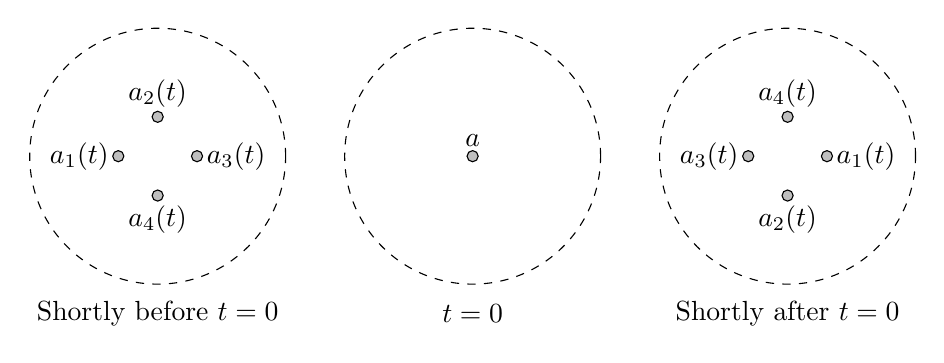
\begin{tikzpicture}[scale=.5]
    \begin{scope}
        \draw[dashed] (0,0) circle (3.25);
        \node[dot] (1) at (180:1) {};
        \node[left] at (1) {$a_1(t)$};
%        \node[left] at (1) {$a_1(-\epsilon)$};
        \node[dot] (2) at (90:1) {};
        \node[above] at (2) {$a_2(t)$};
        \node[dot] (3) at (0:1) {};
        \node[right] at (3) {$a_3(t)$};
        \node[dot] (4) at (270:1) {};
        \node[below] at (4) {$a_4(t)$};
        \node at (0,-4) {Shortly before $t=0$};
    \end{scope}
    \begin{scope}[xshift=8cm]
        \draw[dashed] (0,0) circle (3.25);
        \node[dot] (1) at (0,0) {};
        \node[above] at (1) {$a$};
        \node at (0,-4) {$t=0$};
    \end{scope}
    \begin{scope}[xshift=16cm]
        \draw[dashed] (0,0) circle (3.25);
        \node[dot] (1) at (180:1) {};
        \node[left] at (1) {$a_3(t)$};
        \node[dot] (2) at (90:1) {};
        \node[above] at (2) {$a_4(t)$};
        \node[dot] (3) at (0:1) {};
        \node[right] at (3) {$a_1(t)$};
        \node[dot] (4) at (270:1) {};
        \node[below] at (4) {$a_2(t)$};
        \node at (0,-4) {Shortly after $t=0$};
    \end{scope}
\end{tikzpicture}
\]
\caption{Left centers in a small neighborhood $U$ of $a$}
\label{fig: crossingawall}
\end{figure}

By Proposition \ref{prop: Voronoivertex}, the left centers $a_i(t)$ are vertices of the $k$th order Voronoi decomposition if and only if $C_i(t)$ has $k-2$ or $k-1$ many dots on its left side.
Let $D_-$ denote the dots which are on the left side of $C$; for small enough $\epsilon$, these dots are also on the left side of $C_i(t)$ for all $i\in \{1,2,3,4\}$ and $t\in [-\epsilon,\epsilon]$.

\begin{itemize}
    \item Consider $t\in [-\epsilon,\epsilon]$ for which the dot $d_1(t)$ is on the left side of $C_1(t)$. Then $d_2(t)$ is on the right side of $C_2(t)$, $d_3(t)$ is on the left side of $C_3(t)$, and $d_4(t)$ is on the right side of $C_4(t)$.
    
%     Then the sets of dots on the left of the $C_i(t)$ are below.
% \[
% \begin{array}{|c|c|c|c|c|c|c|c|c|}
% \hline
% \text{Circle} & C_1(t) & C_2(t) & C_3(t) & C_4(t) \\
% \hline
% \text{Dots on left} & D_- \cup \{d_1(t)\} & D_- & D_- \cup \{d_3(t)\} & D_- \\
% \hline
% \end{array}
% \]
    The only way for any of the $a_i(t)$ to be vertices of the $k$th order Voronoi decomposition is if $|D_-|$ is between $k-3$ and $k-1$, in which case the restriction to the neighborhood $U$ will be equivalent to one of the pictures in Figure \ref{fig: d1left}.
    
%    , then the restriction of the $k$th order Voronoi decomposition to $U$ will be equivalent to one of the three pictures in Figure \ref{fig: d1left}. For other values of $|D_-|$, ???

\begin{figure}[h!t]
\[
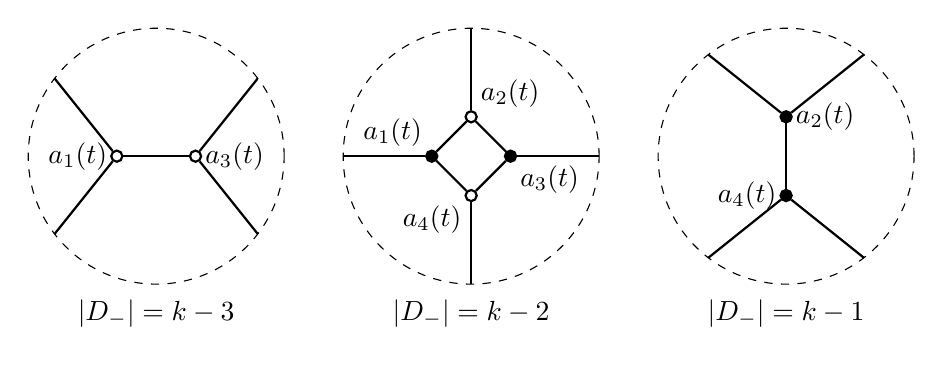
\begin{tikzpicture}[scale=.5]
    \begin{scope}
        \node at (0,-4) {$|D_-|=k-3$};
        \draw[dashed] (0,0) circle (3.25);
        \clip (0,0) circle (3.25);
        \node[dot,thick,fill=white] (1) at (180:1) {};
        \node[left] at (1) {$a_1(t)$};
        % \node[dot] (2) at (90:1) {};
        % \node[above] at (2) {$a_2(t)$};
        \node[dot,thick,fill=white] (3) at (0:1) {};
        \node[right] at (3) {$a_3(t)$};
        % \node[dot] (4) at (270:1) {};
        % \node[below] at (4) {$a_4(t)$};

        \draw[thick] (1) to (3);
        \draw[thick] (1) to (-5,5);
        \draw[thick] (1) to (-5,-5);
        \draw[thick] (3) to (5,5);
        \draw[thick] (3) to (5,-5);
    \end{scope}
    \begin{scope}[xshift=8cm]
        \node at (0,-4) {$|D_-|=k-2$};
        \draw[dashed] (0,0) circle (3.25);
        \clip (0,0) circle (3.25);
        \node[dot,thick,fill=black] (1) at (180:1) {};
        \node[above left] at (1) {$a_1(t)$};
        \node[dot,thick,fill=white] (2) at (90:1) {};
        \node[above right] at (2) {$a_2(t)$};
        \node[dot,thick,fill=black] (3) at (0:1) {};
        \node[below right] at (3) {$a_3(t)$};
        \node[dot,thick,fill=white] (4) at (270:1) {};
        \node[below left] at (4) {$a_4(t)$};

        \draw[thick] (1) to (2);
        \draw[thick] (2) to (3);
        \draw[thick] (3) to (4);
        \draw[thick] (4) to (1);
        \draw[thick] (1) to (-5,0);
        \draw[thick] (2) to (0,5);
        \draw[thick] (3) to (5,0);
        \draw[thick] (4) to (0,-5);
    \end{scope}
    \begin{scope}[xshift=16cm]
        \node at (0,-4) {$|D_-|=k-1$};
        \draw[dashed] (0,0) circle (3.25);
        \clip (0,0) circle (3.25);
        % \node[dot,thick,fill=white] (1) at (180:1) {};
        % \node[left] at (1) {$a_1(t)$};
        \node[dot,thick,fill=black] (2) at (90:1) {};
        \node[ right] at (2) {$a_2(t)$};
        % \node[dot,thick,fill=white] (3) at (0:1) {};
        % \node[right] at (3) {$a_3(t)$};
        \node[dot,thick,fill=black] (4) at (270:1) {};
        \node[ left] at (4) {$a_4(t)$};

        \draw[thick] (2) to (4);
        \draw[thick] (2) to (-5,5);
        \draw[thick] (4) to (-5,-5);
        \draw[thick] (2) to (5,5);
        \draw[thick] (4) to (5,-5);
    \end{scope}
\end{tikzpicture}
\]
\caption{Local structure of $k$th order Voronoi decomp, when $d_1(t)$ is left of $C_1(t)$}
\label{fig: d1left}
\end{figure}
    \item Consider $t\in [-\epsilon,\epsilon]$ for which the dot $d_1(t)$ is on the right side of $C_1(t)$. Then $d_2(t)$ is on the left side of $C_2(t)$, $d_3(t)$ is on the right side of $C_3(t)$, and $d_4(t)$ is on the left side of $C_4(t)$.
    
%     Then the sets of dots on the left of the $C_i(t)$ are below.
% \[
% \begin{array}{|c|c|c|c|c|c|c|c|c|}
% \hline
% \text{Circle} & C_1(t) & C_2(t) & C_3(t) & C_4(t) \\
% \hline
% \text{Dots on left} & D_- \cup \{d_1(t)\} & D_- & D_- \cup \{d_3(t)\} & D_- \\
% \hline
% \end{array}
% \]
    The only way for any of the $a_i(t)$ to be vertices of the $k$th order Voronoi decomposition is if $|D_-|$ is between $k-3$ and $k-1$, in which case the restriction to the neighborhood $U$ will be equivalent to one of the pictures in Figure \ref{fig: d1right}.
    
%    , then the restriction of the $k$th order Voronoi decomposition to $U$ will be equivalent to one of the three pictures in Figure \ref{fig: d1left}. For other values of $|D_-|$, ???

\begin{figure}[h!t]
\[
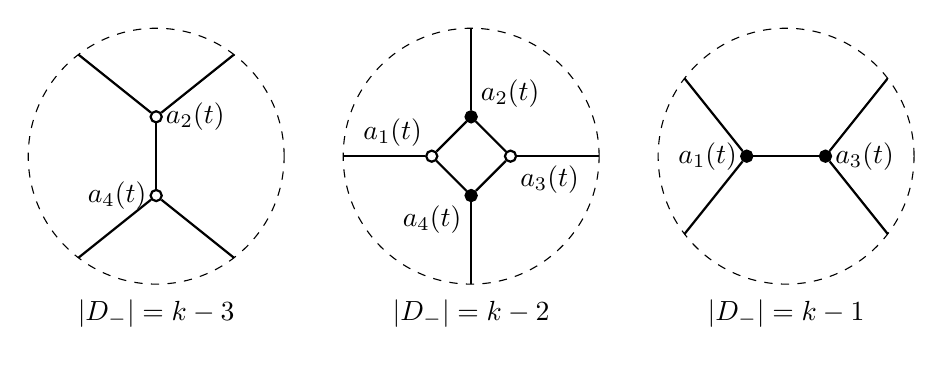
\begin{tikzpicture}[scale=.5]
    \begin{scope}
        \node at (0,-4) {$|D_-|=k-3$};
        \draw[dashed] (0,0) circle (3.25);
        \clip (0,0) circle (3.25);
        % \node[dot,thick,fill=white] (1) at (180:1) {};
        % \node[left] at (1) {$a_1(t)$};
        \node[dot,thick,fill=white] (2) at (90:1) {};
        \node[ right] at (2) {$a_2(t)$};
        % \node[dot,thick,fill=white] (3) at (0:1) {};
        % \node[right] at (3) {$a_3(t)$};
        \node[dot,thick,fill=white] (4) at (270:1) {};
        \node[ left] at (4) {$a_4(t)$};

        \draw[thick] (2) to (4);
        \draw[thick] (2) to (-5,5);
        \draw[thick] (4) to (-5,-5);
        \draw[thick] (2) to (5,5);
        \draw[thick] (4) to (5,-5);
    \end{scope}
    \begin{scope}[xshift=8cm]
        \node at (0,-4) {$|D_-|=k-2$};
        \draw[dashed] (0,0) circle (3.25);
        \clip (0,0) circle (3.25);
        \node[dot,thick,fill=white] (1) at (180:1) {};
        \node[above left] at (1) {$a_1(t)$};
        \node[dot,thick,fill=black] (2) at (90:1) {};
        \node[above right] at (2) {$a_2(t)$};
        \node[dot,thick,fill=white] (3) at (0:1) {};
        \node[below right] at (3) {$a_3(t)$};
        \node[dot,thick,fill=black] (4) at (270:1) {};
        \node[below left] at (4) {$a_4(t)$};

        \draw[thick] (1) to (2);
        \draw[thick] (2) to (3);
        \draw[thick] (3) to (4);
        \draw[thick] (4) to (1);
        \draw[thick] (1) to (-5,0);
        \draw[thick] (2) to (0,5);
        \draw[thick] (3) to (5,0);
        \draw[thick] (4) to (0,-5);
    \end{scope}
    \begin{scope}[xshift=16cm]
        \node at (0,-4) {$|D_-|=k-1$};
        \draw[dashed] (0,0) circle (3.25);
        \clip (0,0) circle (3.25);
        \node[dot,thick,fill=black] (1) at (180:1) {};
        \node[left] at (1) {$a_1(t)$};
        % \node[dot] (2) at (90:1) {};
        % \node[above] at (2) {$a_2(t)$};
        \node[dot,thick,fill=black] (3) at (0:1) {};
        \node[right] at (3) {$a_3(t)$};
        % \node[dot] (4) at (270:1) {};
        % \node[below] at (4) {$a_4(t)$};

        \draw[thick] (1) to (3);
        \draw[thick] (1) to (-5,5);
        \draw[thick] (1) to (-5,-5);
        \draw[thick] (3) to (5,5);
        \draw[thick] (3) to (5,-5);
    \end{scope}
\end{tikzpicture}
\]
\caption{Local structure of $k$th order Voronoi decomp, when $d_1(t)$ is right of $C_1(t)$}
\label{fig: d1right}
\end{figure}
    
\end{itemize}

If $d_1(t)$ switches sides of $C_1(t)$ as $t$ crosses $0$, then the $k$th order Voronoi decomposition changes by one of the local moves in Figure \ref{fig: postnikovmoves}. If $d_1(t)$ stays on the same side of $C_1(t)$ as $t$ crosses $0$, then the $k$th order Voronoi decompositions before and after are equivalent.

%If $k=\frac{1}{2}n$, then $a_i(t)$ is a vertex of the $k$th order Voronoi decomposition if and only if the right center $\sigma(a_i(t)$ of $C_i(t)$ is a vertex, necessarily with the opposite color. Therefore, when $k=\frac{1}{2}n$, whenever t

Next, let $\overline{C}_i(t)$ denote the orientation-reversal of $C_i(t)$ for each $i$. The left center of $\overline{C}_i(t)$ is the right center of $C_i(t)$, which is the antipode $\sigma(a_i(t))$ of the left center $a_i(t)$. Just like Figure \ref{fig: crossingawall}, the four antipodes $\sigma(a_1(p)),\sigma(a_1(p)),\sigma(a_1(p)),\sigma(a_1(p))$ come together to single point $\sigma(a)$ before splitting again, and therefore the Voronoi decomposition changes by a local move or remains equivalent.

For any triple of dots besides the four triples in $\{d_1,d_2,d_3,d_4\}$, the corresponding incident circle does not cross a dot, and therefore has the same set of dots on either side for all $t$. As a consequence, the corresponding vertices in the $k$th order Voronoi decomposition and their adjacencies to other vertices do not change as $t$ varies. Therefore, the $k$th order Voronoi decomposition remains equivalent outside the small neighborhoods of $a$ and $\sigma(a)$.
%
%
% %If $d_1^-$ is on the left side of $C_1^-$ and $d_1^+$ is on the left side of $C_1^+$, then all the same sets of dots on on the same sides of each of the incident circles, and the $k$th order Voronoi decompositions of $D^-$ and $D^+$ are equivalently. Similaly, if $d_1^-$ and $d_1^+$ are both on the right sides, then the $k$th order Voronoi decompositions are equivalent.
%
% Assume that $d_1(-\epsilon)$ is on the left side of $C_1(-\epsilon)$ and $d_1(\epsilon)$ is on the right side of $C_1(\epsilon)$. 
% Let $D_-$ be the set of dots on the left side of $C^0$ and let $D_+$ be the set of dots on the right side of $C^0$. Then 
% \[
% \begin{array}{|c|c|c|c|c|c|c|c|c|}
% \hline
% \text{Circle} & C_1(-\epsilon) & C_2(-\epsilon) & C_3(-\epsilon) & C_4(-\epsilon) & C_1(\epsilon) & C_2(\epsilon) & C_3(\epsilon) & C_4(\epsilon) \\
% \hline
% \text{Dots on left} & D_- \cup \{d_1^-\} & D_- & D_- \cup \{d_3^-\} & D_- & D_- & D_- \cup \{d_2^+\} & D_- & D_- \cup \{d_4^+\} \\
% \hline
% \end{array}
% \]
%
% \begin{itemize}
%     \item If $|D_-|=k-3$, then there are $(k-2)$-many dots on the left side of $C_1^-,C_3^-,C_2^+,C_4^+$, and $(k-3)$-many dots on the left side of $C_2^-,C_4^-, C_1^+,C_3^+$. The $k$th order Voronoi decompositions have white vertices at $a_1^-,a_3^-,a_2^+,a_4^+$ and no vertices at the other left centers. The $k$th order Voronoi decompositions therefore change via the move in Figure \ref{???}.
%     \item If $|D_-|=k-2$, then there are $(k-1)$-many dots on the left side of $C_1^-,C_3^-,C_2^+,C_4^+$, and $(k-2)$-many dots on the left side of $C_2^-,C_4^-, C_1^+,C_3^+$. The $k$th order Voronoi decompositions have black vertices at $a_1^-,a_3^-,a_2^+,a_4^+$ and white vertices at $a_2^-,a_4^-,a_1^+,a_3^+$. The $k$th order Voronoi decompositions therefore change via the move in Figure \ref{???}.
%     \item If $|D_-|=k-1$, then there are $k$-many dots on the left side of $C_1^-,C_3^-,C_2^+,C_4^+$, and $(k-1)$-many dots on the left side of $C_2^-,C_4^-, C_1^+,C_3^+$. The $k$th order Voronoi decompositions have white vertices at $a_2^-,a_4^-,a_1^+,a_3^+$ and no vertices at the other left centers. The $k$th order Voronoi decompositions therefore change via the move in Figure \ref{???}.
%     \item For all other cardinalities of $|D_-|$, none of the left centers are vertices of the $k$th order Voronoi decomposition, and so the Voronoi decomposition does not change from $D$ to $D'$.
% \end{itemize}
%
% If $d_1^-$ is on the right side of $C_1^-$ and $d_1^+$ is on the left side of $C_1^+$, then reversing the direction of the parameterization reduces to the previous case, and the $k$th order Voronoi decompositions change via the moves in the other direction.
%
% Consider a semigeneral family $D(t)$ which is general except at $t=0$. Let $d_1^0,d_2^0,d_3^0,d_4^0$ be the unique quadruple of dots that are colinear at $t=0$ (indexed in circular order), and let $C$ denote the incident circle through those four dots. Let $d_i^+$ and $d_i^$ denote these points for arbitrarily small positive and negative values of $t$.
%
% Let $C_1^t$ denote the oriented circle through $d_2^t,d_3^t,d_4^t$; similarly, let $C_2^t, C_3^t,C_4^t$ denote the family of oriented circles the other three triples.
% If $d_1^-$ is on the left of $C_1^-$ and $d_1_+$ is on the left of $C_1^+$,
\end{proof}

\begin{rem}
The proof demonstrates that moves occur in pairs only when $k$ is close to $\frac{1}{2}n$. When $k=\frac{1}{2}n$, then every move must occur in antipodal pairs (to preserve the symmetry from Proposition \ref{prop: antipodal}). When $n=2k\pm1$, then only some moves will occur in pairs; specifically, every square move will be accompanied by one of the merging-splitting moves.
\end{rem}


%
Proposition \ref{prop: semigeneral} and Lemma \ref{lemma: move} immediately imply the following.

\begin{rethm}{\ref{thm: move equiv}}
Let $0<k<n>3$. The $k$th order Voronoi decompositions of any two sets of $n$-many dots in general position in the sphere may be related by a sequence of the local moves in Figure \ref{fig: postnikovmoves}.
% Let $0<k<n>3$,
% any two configurations of $n$-many dots in general position in the sphere have move-equivalent $k$th order Voronoi decompositions.
%Any two $k$th order Voronoi decompositions of the sphere are move-equivalent.
\end{rethm}

The moves in Figure \ref{fig: postnikovmoves} between bicolored graphs appeared in the seminal work of Postnikov, where such moves induced an equivalence between many associated constructions, such as \emph{boundary measurement maps}, \emph{trip permutations}, and \emph{cluster algebras}. While the first two constructions do not have an obvious generalization to bicolored graphs in the sphere, we briefly consider the associated cluster algebra in Section \ref{sec: future}. %Following Postnikov, we say two bicolored graphs in the sphere are \textbf{move-equivalent} if they may be related by a finite sequence of the local moves in Figure \ref{fig: postnikovmoves}.

\begin{rem}
Theorem \ref{thm: move equiv} provides a second proof that the numbers of black vertices, white vertices, edges, and regions in a spherical $k$th order Voronoi decomposition only depends on $k$ and $n$, since the local moves preserve these counts. While it doesn't provide any counts, one could pick a particular nice configuration and count strata there to (re)deduce the formulas in Theorem \ref{thm: stratacount}. A proof in this spirit of the $k=\ell$ case of  Theorem \ref{thm: incident} is given in \cite{Ard04}.
\end{rem}

\begin{warn}
We caution the reader that some Postnikov moves cannot be realized by a semigeneral family! The most obvious obstruction is that, when $k=\frac{1}{2}n$, the $k$th order Voronoi decomposition is antipodally symmetric, and so semigeneral homotopies \emph{must} induce local moves in antipodal pairs. However, one may construct counterexamples for other values of $k$ as well.
\end{warn}

\section{Future directions}\label{sec: future}

We close by sketching some of the further directions one may take these ideas in, particularly those directions opened up by Theorem \ref{thm: move equiv}.

In \cite{Pos}, the author shows how a bicolored graph in a surface can be used to define a \emph{cluster algebra}, a special kind of commutative ring with distinguished elements called \emph{cluster variables} (a more modern exposition of this construction can be found in \cite{FWZdd}).
Given a configuration $D$ of $n$-many dots in general position in the sphere $S$, 
let $\mathcal{A}_\circlearrowleft(k,D)$ denote the cluster algebra associated to the $k$th order Voronoi decomposition of $S$ determined by $D$.

Since the moves in Figure \ref{fig: postnikovmoves} each induce an isomorphism between the associated cluster algebras \cite[Proposition 7.2.2]{FWZdd}, Theorem \ref{thm: move equiv} immediately implies the following.

\begin{prop}
Let $0<k<n>3$, and let $D, D'$ be configurations of $n$-many dots in general position in $S$.
Then a semigeneral family from $D$ to $D'$ induces an isomorphism of cluster algebras
\[
\mathcal{A}_\circlearrowleft(k,D) \rightarrow \mathcal{A}_\circlearrowleft(k,D')
\]
In particular, the isomorphism class of $\mathcal{A}_\circlearrowleft(k,D)$ only depends on $k$ and $n$.
\end{prop}

As we hope to show in a future work, this isomorphism only depends on the semigeneral family up to homotopy in $\Conf_n(S)$. As a consequence, elements in the fundamental group
\[
\pi_1(\Conf_n(S),D)
\]
induce well-defined automorphisms of $\mathcal{A}_\circlearrowleft(k,D)$. This fundamental group is called the \emph{$n$th spherical braid group}, and it can be identified with the \emph{mapping class group of the punctured sphere $S\smallsetminus D$}. Using this action, one can show that every homotopy class of simple, \emph{oriented} curve in $S\smallsetminus D$ with $k$-many dot on its left side determines a cluster variable in $\mathcal{A}_\circlearrowleft(k,D)$.%; note that such curves realizable by circles are precisely the \emph{initial} cluster variables.

% \[
% \{\text{oriented curves in $S\smallsetminus D$ with $k$-many dots on their left side}\}/\text{homotopy}
% \rightarrow 
% \{\text{cluster variables in $\mathcal{A}(k,D)$}\}
% \]

This suggests a natural variant for unoriented curves. Recall that, when $2k=|D|$, the $k$th order Voronoi decomposition has an antipodal symmetry. Let $\mathcal{A}_\bigcirc(k,D)$ be the cluster algebra of the quotient of this Voronoi decomposition by the antipodal symmetry\footnote{Or equivalently, as a \emph{fold} of the cluster algebra $\mathcal{A}_\circlearrowleft(k,D)$ by the antipodal symmetry (in the sense of \cite{Dup08}).}; for all other choices of $k$, let $\mathcal{A}_\bigcirc(k,D) :=\mathcal{A}_\circlearrowleft(k,D)$.  As before, the isomorphism class of $\mathcal{A}_\bigcirc(k,D)$ only depends on $k$ and $n:=|D|$, and one can show that every homotopy class of simple, \emph{unoriented} curve in $S\smallsetminus D$ with $k$-many dots on one of its sides determines a cluster variable in $\mathcal{A}_\bigcirc(k,D)$.

\begin{rem}
For small values of $n$, the cluster algebras $\mathcal{A}_\bigcirc(k,D)$ are of special and notable types. 

When $|D|=4$, the $\mathcal{A}_\bigcirc(2,D)$ is isomorphic to the \emph{Markov cluster algebra} \cite{BFZ05}, which is related to the Teichm\"uller space of the once-punctured torus and the theory of Markov triples. 

When $|D|=6$, the cluster algebra $\mathcal{A}_\bigcirc(3,D)$ is isomorphic to the \emph{$X_7$ cluster algebra}, an exotic and largely mysterious cluster algebra which appears as one of two sporadic cases in the classification of \emph{mutation-finite} cluster algebras \cite{DO08}. This realization (particularly, the action of the mapping class group) has non-trivial consequences for the structure of this cluster algebra, as well as for the combinatorics of separating curves in the closed surface of genus 2. We hope to explore these consequences in a future work.
\end{rem}

% \begin{figure}[h!t]
% \[
% \begin{array}{|c|c|c|c|}
% (k,n) & \text{Type of }\mathcal{A}(k,n) \\
% \hline
% (1,n) & \text{Toric (no mutable variables)} \\
% (2,n) & 
% \end{array}
% \]
% \end{figure}

\appendix

\section{Connection between spherical and planar Voronoi decompositions}\label{appendix}

A curious feature of our proofs of Theorems \ref{thm: incident} and \ref{thm: avoidant} is they are both fundamentally spherical, even though the ultimate results are equally valid in the sphere and the plane.
%
One explanation is that our proofs boil down to counting various strata in the $k$th order Voronoi decomposition of the sphere (Theorem \ref{thm: stratacount}), and stereographic projection does \emph{not} send Voronoi decompositions to Voronoi decompositions. %This can be seen in Figure \ref{fig: stereoVoronoi}, where the stereographic projection of a $2$nd order Voronoi decomposition 
While stereographic projection sends circles to circles, it does not send the center of a circle to the center of its image.

However, there is a more subtle relationship between higher order Voronoi decompositions in the plane and sphere, which we sketch here for the benefit of the reader. In essence, the spherical $k$th order Voronoi decomposition can be constructed by gluing together the planar $k$th order Voronoi decomposition and the planar $(n-k)$th order Voronoi decomposition.

\begin{thm}[\cite{Brown79,NLC02,CHP22}]
Let $D$ be a configuration of dots in the sphere $S$, and let $\pi(D)$ be the stereographic projection in the plane $P$.%, and consider the corresponding higher order Voronoi decompositions.
\begin{enumerate}
    \item There is a simple, piecewise-circular curve $R_0$ in $S$, disjoint from the vertices of the $k$th order Voronoi decomposition of $S$ determined by $D$, whose complement consists of two open regions $R_+$ and $R_-$.
    \item There is a homeomorphism from $R_+$ to the plane $P$ which induces a color-preserving equivalence between the $k$th order Voronoi decomposition of $S$ determined by $D$ (as restricted to $R_+$) and the $k$th order Voronoi decomposition of $P$ determined by $\pi(D)$.
    \item There is a homeomorphism from $R_-$ to the plane $P$ which induces a color-swapping equivalence between the $k$th order Voronoi decomposition of $S$ determined by $D$ (as restricted to $R_-$) and the $(n-k)$th order Voronoi decomposition of $P$ determined by $\pi(D)$.
\end{enumerate}
\end{thm}

The first version of this appeared in \cite{Brown79}, who proved parts (1) and (2) for $k=1$ to derive ($k=1$) Voronoi decompositions in the plane from (computationally faster) ($k=1$) Voronoi decompositions in the sphere. Part (3) of the $k=1$ case was shown in \cite{NLC02} with explicit maps. The general $k$ version appears in \cite{CHP22}, who used it to deduce the number of incident and avoidant circles from analogous results on planar Voronoi decompositions due to \cite{Lin03}.

\begin{rem}
The theorem implies that the number of white vertices in a spherical $k$th order Voronoi decomposition is equal to the number of white vertices in the corresponding planar $k$th order Voronoi decomposition plus the number of black vertices in the planar $(n-k)$th order Voronoi decomposition. Translating into circles, this is equivalent to a simple observation: given a configuration of $n$-many dots in general position in the plane, the number of incident circles with $(k-2)$-many dots on either side is equal to the number of incident circles with $(k-2)$-many dots in the interior plus the number of incident circles with $(n-k-1)$-many dots in the interior.
\end{rem}

%This idea appears to originate in Brown's dissertation \cite{???} who used it to relate classical ($k=1$) Voronoi decompositions in the plane and sphere. The 

% \begin{warn}
% The reader is cautioned that the curve $R_0$ is generally not smooth; rather, it is piecewise circular, and the homeomorphisms from $R_\pm$ to $P$ are only piecewise stereographic. 
% \end{warn}


\bibliographystyle{alpha}
\bibliography{circles}

\end{document}
